\exercisegroup

\begin{enumerate}
\def\labelenumi{\arabic{enumi})}
\item
  Let I be an uncountable set, and let E be the space \(\mathbf{R}^{(I)}\) endowed with the topology defined in I, p.~24, exerc. 14; let \(E'\) be its dual (IV, p.~50, exerc. 16, c)). Show that in \(E'\) there exist non relatively compact (for \(\sigma(E', E)\) ) subsets H such that from every sequence of points of H we can extract a sequence which converges to a point of H for \(\sigma(E', E)\) .
\item
  \begin{enumerate}
  \def\labelenumii{\alph{enumii})}
  \tightlist
  \item
    Let X be a regular space and A a subset of X. Suppose that every sequence of points of A has a limit point in X and that there exists a metrizable topology T on X which is coarser than the given topology \(T_{0}\) . Show that the closure \(\overline{A}\) of A in X is a compact metrizable space (arguing by reductio ad absurdum, show that the topologies induced by T and \(T_{0}\) on \(\overline{A}\) are identical).
  \end{enumerate}
\end{enumerate}

\begin{enumerate}
\def\labelenumi{\alph{enumi})}
\setcounter{enumi}{1}
\item
  Let E be a Hausdorff locally convex space, which is the union of a sequence \((\mathrm{E}_{n})\) of metrizable vector subspaces for the topology induced by that of E. Show that, for a subset A of E to be relatively compact in E, it is necessary and sufficient that every sequence of points of A has a limit point in E. (If \((\mathrm{W}_{mn})\) (for \(m \geqslant 1\) ) is a fundamental system of convex neighbourhoods of 0 in \(E_{n}\) which are open in \(E_{n}\) , let \(U_{mn}\) be a convex neighbourhood of 0 in E such that \(E_{n} \cap U_{mn} = W_{mn}\) (II, p.~33, lemma 2); on E consider the topology for which the \(U_{mn}\) ( \(m \geqslant 1\) , \(n \geqslant 1\) ) form a fundamental system of neighbourhoods of 0).
\item
  Extend Šmulian's theorem to a strict inductive limit space (II, p.~33) of Fréchet spaces.
\end{enumerate}

\begin{enumerate}
\def\labelenumi{\arabic{enumi})}
\setcounter{enumi}{2}
\tightlist
\item
  \begin{enumerate}
  \def\labelenumii{\alph{enumii})}
  \tightlist
  \item
    Let E be a Hausdorff locally convex space and \(E'\) its dual; suppose that there exists a countable everywhere dense set in \(E'\) for the topology \(\sigma(E', E)\) . Show that the topology of E (resp. \(\sigma(E, E')\) ) is finer than a metrizable locally convex topology.
  \end{enumerate}
\end{enumerate}

\begin{enumerate}
\def\labelenumi{\alph{enumi})}
\setcounter{enumi}{1}
\item
  Let \((x_{n})\) be a sequence of points of E such that every sequence extracted from \((x_{n})\) has a limit point for the initial topology (resp. the topology \(\sigma (\mathrm{E},\mathrm{E}^{\prime})\) ). Show that there exists a sequence extracted from \((x_{n})\) which converges in E for the initial topology (resp. the topology \(\sigma (\mathrm{E},\mathrm{E}^{\prime})\) ). (Let \((a_n^{\prime})\) be an everywhere dense sequence in \(\mathbf{E}'\) for \(\sigma (\mathrm{E}',\mathrm{E})\) ; extract a sequence \((y_{n})\) from \((x_{n})\) such that \((\langle y_n,a_p'\rangle)\) tends to a limit for every index \(p\) , and show that the sequence \((y_{n})\) has only one limit point for the initial topology (resp. for \(\sigma (\mathrm{E},\mathrm{E}^{\prime}))\) .)
\item
  For a subset A of E to be relatively compact for the initial topology (resp. for \(\sigma(E, E')\) , it is necessary and sufficient that from every sequence \((x_n)\) of points of A, we can extract a sequence \((x_{n_k})\) which converges to a point of E for the initial topology (resp. for \(\sigma(E, E')\) ) (use exerc. 2, a)).
\end{enumerate}

\begin{enumerate}
\def\labelenumi{\arabic{enumi})}
\setcounter{enumi}{3}
\item
  Let \(\mathrm{E}\) be the Banach space \(l^{\infty}(\mathbb{N})\), which does not satisfy the first axiom of countability (I, p.~25, exerc. 1), and let \(\mathrm{E}'\) be its dual. For every integer \(n \geqslant 0\) , let \(e_n'\) be the continuous linear form on E which associates to each \(x = (\xi_n) \in \mathrm{E}\) the \(n\) th term of this sequence. Show that the sequence \((e_n')\) is total in \(\mathrm{E}'\) for \(\sigma(\mathrm{E}', \mathrm{E})\) ; moreover, every sequence extracted from \((e_n')\) has a limit point in \(\mathrm{E}'\) , for the topology \(\sigma(\mathrm{E}', \mathrm{E})\) , but there exists no sequence extracted from \((e_n')\) which converges in \(\mathrm{E}'\) for this topology.
\item
  \begin{enumerate}
  \def\labelenumii{\alph{enumii})}
  \tightlist
  \item
    Let X be a compact space, H an arbitrary subset of the space \(\mathcal{C}(\mathrm{X})\) of continuous numerical functions on X. Let \(f_{0}\) be a point of \(\mathcal{C}(\mathrm{X})\) which is in the closure of H for the topology \(T_{s}\) of simple convergence on \(\mathcal{C}(\mathrm{X})\) . Show that there exists a countable subset \(H_{0}\) of H such that \(f_{0}\) is in the closure of \(H_{0}\) for \(T_{s}\) . (Show that for every pair of integers m \textgreater{} 0, n \textgreater{} 0 there exists a finite subset \(\mathrm{H}(m, n)\) of H with the following property: for every set of m points \(t_{k}\) in X ( \(1 \leqslant k \leqslant m\) ), there exists \(f \in \mathrm{H}(m, n)\) such that \(|f_{0}(t_{k}) - f(t_{k})| \leqslant 1/n\) for \(1 \leqslant k \leqslant m\) . b) Let E be a locally convex metrizable space, \(E'\) its dual and H a subset of E. Show that if \(x_{0}\) is in the closure of H for the weakened topology \(\sigma(\mathrm{E}, \mathrm{E}')\) , then there exists a countable subset \(H_{0}\) of H such that \(x_{0}\) is in the closure of \(H_{0}\) for this topology. (Use a), observing that \(E'\) is the union of a countable family of compact sets for \(\sigma(\mathrm{E}', \mathrm{E})\) .)
  \end{enumerate}
\end{enumerate}

¶ 6) a) Let X be a compact space, H a convex subset of the product space \(\mathbf{R}^{\mathrm{X}}\) , consisting of continuous functions on X. Suppose that every decreasing sequence of non-empty convex and closed subsets in H has a non-empty intersection. Show that the closure \(\overline{\mathrm{H}}\) of H in \(\mathbf{R}^{\mathrm{X}}\) is compact and consists of continuous functions on X. (Argue by reductio ad absurdum: consider a non continuous function \(u \in \overline{\mathrm{H}}\) ; show that then there will exist a point \(a \in \mathrm{X}\) , a number \(\delta > 0\) , a sequence \((x_{n})\) points of X and a sequence \((f_{m})\) of functions in H such that:

\(1^{\circ}\left|u(x_{n}) - u(a)\right|\geqslant \delta\) for all \(n;2^{\circ}\left|f_{m}(x_{n}) - f_{m}(a)\right|\leqslant \frac{\delta}{8}\) for \(m\leqslant n;3^{\circ}\left|u(x_{n}) - f_{m}(x_{n})\right|\leqslant \frac{\delta}{8}\) and

\(\left|u(a) - f_m(a)\right| \leqslant \frac{\delta}{8}\) for \(m \geqslant n + 1\) . Consider a limit point \(b\) of the sequence \((x_n)\) , and a function \(f\) belonging to the intersection of the \(\mathbf{A}_m\) , where \(\mathbf{A}_m\) is the closed convex envelope in \(\mathbf{H}\) of the set of all \(f_k\) for \(k \geqslant m\) .

\begin{enumerate}
\def\labelenumi{\alph{enumi})}
\setcounter{enumi}{1}
\tightlist
\item
  Let E be a Hausdorff and quasi-complete locally convex space, \(E'\) its dual. Let H be a convex subset of E such that every decreasing sequence of non-empty and closed convex subsets of H has a non-empty intersection; show that H is relatively compact in E for the topology \(\sigma(\mathrm{E}, \mathrm{E}')\) . (Reduce to the case where E is complete; consider E to be embedded in \(E'^{*}\) and use a) and also III, p.~21, cor. 1.)
\end{enumerate}

\begin{enumerate}
\def\labelenumi{\arabic{enumi})}
\setcounter{enumi}{6}
\item
  Let \(\mathbf{E}\) be a Fréchet space satisfying the first axiom of countability, \(\mathbf{E}'\) its dual. Show that for a convex subset \(\mathbf{A}'\) of \(\mathbf{E}'\) to be closed for \(\sigma(\mathbf{E}', \mathbf{E})\) , it is sufficient that, if a sequence \((x_n')\) of points of \(\mathbf{A}'\) has a limit \(a'\) in \(\mathbf{E}'\) for \(\sigma(\mathbf{E}', \mathbf{E})\) , then \(a' \in \mathbf{A}'\) .
\item
  Let \(\mathrm{F}\) and \(\mathrm{G}\) be two vector spaces in separating duality. Show that the properties \(\alpha)\) and \(\beta)\) of IV, p.~52, exerc. 6, a) are also equivalent to the following:
\end{enumerate}

\(\gamma)\) F, with \(\tau (\mathrm{F},\mathrm{G})\) is quasi-complete, and every bounded sequence of points of F has a limit point for \(\sigma (\mathrm{F},\mathrm{G})\) (cf.~IV, p.~35, th. 1);

δ) F, with \(\tau(\mathrm{F},\mathrm{G})\) is quasi-complete, and every decreasing sequence of non-empty closed convex and bounded sets in F has a non-empty intersection (cf.~exerc. 6, b)).

\begin{enumerate}
\def\labelenumi{\arabic{enumi})}
\setcounter{enumi}{8}
\tightlist
\item
  Let E be a Hausdorff and quasi-complete locally convex space; for E to be semi-reflexive, it is necessary and sufficient that every closed vector subspace of E, in which there exists a countable everywhere dense subset, is semi-reflexive (cf.~IV, p.~35, th. 1).
\end{enumerate}

¶ 10) Let E be a Hausdorff, quasi-complete and non semi-reflexive locally convex space, and let H be a closed hyperplane in E containing the origin. Let \((\mathbf{C}_{n})\) be a decreasing sequence of non-empty, closed convex and bounded sets, contained in H and not containing 0 and whose intersection is empty (exerc. 8). Let x be a point not belonging to H, and let A be the closed

convex and balanced envelope of the union of the sets \(\left(1 - \frac{1}{n}\right)x + C_n\) for \(n > 0\) .

\begin{enumerate}
\def\labelenumi{\alph{enumi})}
\item
  Show that there exists no supporting hyperplane of A which is parallel to H (for \(y \in x + H\) , observe that there exists an integer n such that \(y \notin x + C_{n}\) ).
\item
  Let \(z \in \mathbf{H}\) be such that \(z \notin \mathbf{C}_1\) ; show that the convex envelope of the union of two closed convex and bounded sets \(\mathbf{A}\) and \(\mathbf{B} = x + z + \mathbf{C}_1\) , is not closed (prove that \(x + z\) is in the closure of this envelope, but does not belong to it).
\end{enumerate}

\begin{enumerate}
\def\labelenumi{\arabic{enumi})}
\setcounter{enumi}{10}
\item
  Let A be an infinite set, and let \(E = \overline{\mathcal{H}}(A)\) (IV, p.~47, exerc. 1), \(E' = \ell^{1}(A)\) its dual, \(E'' = \ell^{\infty}(A)\) its bidual (IV, p.~54, exerc. 14). Show that every subset of \(E'\) , which is compact for \(\sigma(E', E'')\) is strongly compact (use Šmulian's theorem and IV, p.~54, exerc. 15).
\item
  Let E be a non reflexive Banach space. Prove that there exists a closed, non reflexive vector subspace M of infinite codimension in E. (Let \((x_{n})\) be a bounded sequence in E which has no limit point for the topology \(\sigma(\mathrm{E},\mathrm{E}')\) (IV, p.~68, exerc. 8); by induction construct a sequence \((x_{n_{k}})\) extracted from \((x_{n})\) and a topologically free sequence \((y_{k})\) such that \(\| x_{n_{k}} - y_{k} \| \leqslant 1/k\) for \(k \geqslant 1\) , and consider the closed vector subspace of E generated by the \(y_{2k}\) .
\end{enumerate}

¶ 13) Let E be a non reflexive Banach space satisfying the first axiom of countability, and let M be a non reflexive closed vector subspace of E of infinite codimension (exerc. 12). Let \((x_{n})\) be an everywhere dense sequence in the unit sphere, C the closed convex balanced envelope of the sequence \((x_{n}/n)\) ; C is strongly compact in E and \(C + M = A\) is a closed convex set (GT, III, § 4, No.~1, cor. 1 to prop. 1). Let S be the unit ball in E, and \(B = A \cap S\) .

\begin{enumerate}
\def\labelenumi{\alph{enumi})}
\item
  Show that 0 is not an interior point of A and deduce that there exists \(x_0 \in E\) such that \(\lambda x_0 \notin A\) for \(\lambda > 0\) .
\item
  Show that there exists no supporting hyperplane of B passing through 0 (observe that such a hyperplane must be a supporting hyperplane of C).
\item
  Let \(\mathrm{U}_0 = \mathrm{M} \cap \mathrm{S}\) , and let \((\mathrm{U}_n)_{n \geqslant 1}\) be a decreasing sequence of closed convex, bounded and non-empty sets, such that \(\mathrm{U}_1 \subset \frac{1}{2}\mathrm{U}_0\) and such that the intersection of the \(\mathrm{U}_n\) is empty (IV, p.~68, exerc. 8). Let \(\mathbf{F}\) be the closed convex envelope of the union of the sets \(\frac{1}{n} x_0 + \mathrm{U}_n\) ( \(n \geqslant 1\) ). Show that \(\mathbf{B} \cap \mathbf{F} = \emptyset\) but that there exists no closed hyperplane separating \(\mathbf{B}\) and \(\mathbf{F}\) (use \(b\) )).
\end{enumerate}

\begin{enumerate}
\def\labelenumi{\arabic{enumi})}
\setcounter{enumi}{13}
\tightlist
\item
  Let \(\mathbf{E}\) be a Banach space satisfying the first axiom of countability. A sequence \((e_n)_{n\geqslant 0}\) of elements of \(\mathbf{E}\) is said to be a Banach basis if the following property is satisfied: for every \(x\in \mathbb{E}\) , there exists a unique sequence \((a_{n})\) of scalars such that \(x = \sum_{n = 0}^{\infty}a_{n}e_{n}\) , where the series on
\end{enumerate}

the right hand side is convergent.

\begin{enumerate}
\def\labelenumi{\alph{enumi})}
\tightlist
\item
  Show that the family \((e_n)\) is total and free. Let \(E_n\) be the vector subspace (closed) of E generated by the \(e_m\) for indices \(m \leqslant n\) , and let \(P_n\) be the projector from E onto \(E_n\) defined by \(P_n \cdot (\sum_{m=0}^{\infty} a_m e_m) = \sum_{m=0}^{n} a_m e_m\) . Show that the \(P_n\) are continuous linear mappings and that
\end{enumerate}

\(\sup_{n}\| P_{n}\| < + \infty .\) (Consider the norm on E defined by \(\left\| \sum_{n = 0}^{\infty}a_n e_n\right\| = \sup_{n}\left\| \sum_{m = 0}^{n}a_me_m\right\|\)

show that E is complete for this norm and deduce that it is equivalent to the given norm on E (cf.~I, p.~17, th. 1).) Show that for every pair of integers \(p < q\) , the norm of the projection \(P_{q,p}\) of \(\mathrm{E}_q\) onto \(\mathrm{E}_p\) , which is parallel to the vector subspace generated by the \(e_m\) for indices \(m\) such that \(p + 1 \leqslant m \leqslant q\) , is bounded by a number independent of \(p, q\) .

\begin{enumerate}
\def\labelenumi{\alph{enumi})}
\setcounter{enumi}{1}
\tightlist
\item
  Conversely, let \((e_{n})\) be a total sequence of elements of E, which is a free family and is such that the norms of the projections \(P_{q,p}\) for \(0 \leqslant p < q\) are bounded by a number M independent of p and q. Show that \((e_{n})\) is a Banach basis of E. (First prove that the sequence \((e_{n})\) is topologically free and define the projectors \(P_{n}\) ; then \(\|P_{n}\| \leqslant M\) for all n.~Next observe that if \(d(x, E_{n})\) is the distance of a point \(x \in E\) from \(E_{n}\) , then \(\|x - P_{n} \cdot x\| \leqslant (M + 1) d(x, E_{n})\) .) \(^{1}\)
\end{enumerate}

\(^{1}\) It is clear that the existence of a Banach basis in E implies that E satisfies the first axiom of countability. But there are examples of Banach spaces satisfying the first axiom of countability in which there does not exist a Banach basis (P. ENFLO, Acta Math., t. CXXX (1973), p.~309-317).

¶ 15) Let E be a Banach space with a Banach basis \((e_n)\) (exerc. 14); then there exists a unique sequence \((e_n')\) in the dual \(E'\) of E such that the expression of every \(x \in E\) in terms of the Banach basis \((e_n)\) can be written as \(x = \sum_{n=0}^{\infty} \langle x, e_n' \rangle e_n\) .

\begin{enumerate}
\def\labelenumi{\alph{enumi})}
\item
  Let \(\mathrm{F}_n\) be the closed vector subspace of \(\mathbf{E}\) generated by the \(e_m\) for \(m \geqslant n\) . For every \(x' \in \mathbf{E}'\) , let \(\| x' \|_n\) denote the norm of the restriction of the linear form \(x'\) to \(\mathrm{F}_n\) . Show that, for \((e_n')\) to be a Banach basis of \(\mathbf{E}'\) , it is necessary and sufficient that for every \(x' \in \mathbf{E}'\) , the sequence \((\| x' \|_n)\) tends to 0. (Consider the transpose \({}^t P_n\) and evaluate the norm \(\| {}^t P_n \cdot x' - x' \|\) .) In this case, the Banach basis \((e_n)\) is said to be contracting.
\item
  Suppose that the Banach basis \((e_n)\) is contracting. Show that for every point \(x''\) of the bidual \(\mathrm{E}''\) of E, the sequence of sums \(\sum_{m=0}^{n} \langle e_m', x'' \rangle e_m\) is bounded in E (consider the transpose \(t^t P_n\) )
\end{enumerate}

in \(\mathrm{E}''\) ). Conversely, for every sequence \((a_{n})\) of scalars such that the sequence of sums \(\sum_{m=0}^{n} a_{m} e_{m}\)

is bounded in E, there exists a unique \(x'' \in E''\) such that \(\langle e_{n}', x'' \rangle = a_{n}\) for all n (use the compactness of a closed ball in \(E''\) for the topology \(\sigma(E'', E')\) ).

\begin{enumerate}
\def\labelenumi{\alph{enumi})}
\setcounter{enumi}{2}
\item
  A Banach basis \((e_n)\) in E is said to be complete if, for every sequence \((a_n)\) of scalars such that the sequence of sums \(\sum_{m=0}^{n} a_m e_m\) is bounded, the series \(\sum_{n=0}^{\infty} a_n e_n\) converges. If \((e_n)\) is a contracting basis of E, the basis \((e_{n}^{\prime})\) of \(E^{\prime}\) is complete (use the compactness of a closed ball in \(E^{\prime}\) for \(\sigma(\mathrm{E}^{\prime},\mathrm{E})\) ). d) In general, the sequence \((e_{n}^{\prime})\) is a Banach basis of the closed subspace \(F^{\prime}\) of the strong dual \(E^{\prime}\) of E, generated by the \(e_{n}^{\prime}\) , and there is an injective continuous linear mapping J from E into the strong dual \(F^{\prime\prime}\) of \(F^{\prime}\) such that \(\langle J.x,z^{\prime}\rangle=\langle x,z^{\prime}\rangle\) for all \(x\in E\) and all \(z^{\prime}\in F^{\prime}\) . Show that there exists a constant K\textgreater0 such that \(\|J.x\|\geqslant K.\|x\|\) , and that if the basis \((e_{n})\) is complete, then J is an isomorphism from E onto the topological vector space \(F^{\prime\prime}\) .
\item
  Show that for \(\mathbf{E}\) to be reflexive, it is necessary and sufficient that the basis \((e_n)\) is contracting and complete (use \(b\) ).
\end{enumerate}

\begin{enumerate}
\def\labelenumi{\arabic{enumi})}
\setcounter{enumi}{15}
\tightlist
\item
  \begin{enumerate}
  \def\labelenumii{\alph{enumii})}
  \tightlist
  \item
    Let \(\mathbf{E}\) be a Banach space. For an infinite sequence \((x_{n})\) of points of \(\mathbf{E}\) , the following properties are equivalent:
  \end{enumerate}
\end{enumerate}

\(\alpha)\) The series with the general term \(x_{n}\) is commutatively convergent (GT, III, § 5, No.~7).

\(\beta)\) For every subset I of \(\mathbf{N}\) , the series defined by the sequence \((x_{n})_{n\in \mathrm{I}}\) is convergent (GT, III, § 5, No.~3, prop. 2 and § 5, exerc. 4).

\(\gamma)\) For every sequence \((\varepsilon_{n})\) of numbers equal to 1 or to \(-1\) , the series with the general term \(\varepsilon_{n}x_{n}\) is convergent.

\(\delta)\) For every \(\varepsilon > 0\) , there exists a finite subset \(J\) of \(N\) such that, for every finite subset \(H\) of \(N\) not intersecting \(J\) , we have \(\| \sum x_n \| \leqslant \varepsilon\) .

\begin{enumerate}
\def\labelenumi{\alph{enumi})}
\setcounter{enumi}{1}
\tightlist
\item
  Let \((e_n)\) be a Banach basis of E. The following properties are equivalent:
\end{enumerate}

\(\alpha)\) For every permutation \(\pi\) of \(\mathbf{N}\) , the sequence \((e_{\pi(n)})\) is a Banach basis of E.

\(\beta)\) For every sequence \((\varepsilon_{n})\) of numbers equal to 1 or to -1, the sequence \((\varepsilon_{n}e_{n})\) is a Banach basis of E.

\(\gamma)\) For every \(x = \sum_{n=0}^{\infty} \xi_n e_n\) in E and every sequence \((\eta_n)_{n \in \mathbb{N}}\) for which \(|\eta_n| \leqslant |\xi_n|\) for all \(n\) , the series with the general term \(\eta_n e_n\) converges in E.

δ) For every \(x = \sum_{n=0}^{\infty} \xi_n e_n\) in E and every strictly increasing sequence \((n_k)_{k \in \mathbf{N}}\) of integers \(\geqslant 0\) , the series with the general term \(\xi_{n_k} e_{n_k}\) converges in E.

ε) There exists a real number M \textgreater{} 0 such that, for every finite subset J of N and for every \(x = \sum_{n=0}^{\infty} \xi_{n} e_{n}\) in E, we have \(\left\|\sum_{n \in J} \xi_{n} e_{n}\right\| \leqslant M \|x\|\) .

(To prove that \(\alpha\) ) implies \(\varepsilon\) ), argue as in IV, p.~69, exerc. 14. To prove that \(\beta\) implies \(\gamma\) ), reduce to the case where the \(\xi_{n}\) and the \(\eta_{n}\) are real, and consider the sums \(\sum_{n=p}^{q} \langle \eta_{n} e_{n}, x' \rangle\) for \(x' \in E'\) .)

When these conditions are satisfied, \((e_n)\) is said to be an unconditional Banach basis of E. c) Suppose \((e_n)\) is an unconditional basis. Show that there exists a real number \(K > 0\) such that, for every sequence \((\varepsilon_n)\) of numbers equal to 1 or -1 and for all \(x = \sum_{n=0}^{\infty} \xi_n e_n\) in E, we have \(\| \sum_{n=0}^{\infty} \varepsilon_n \xi_n e_n \| \leqslant M \| x\|\) (same method as in IV, p.~69, exerc. 14). Deduce that for every

bounded sequence of scalars \((\lambda_{n})\) and for all \(x = \sum_{n=0}^{\infty} \xi_{n} e_{n}\) in X, we have

\[
\left\| \sum_ {n = 0} ^ {\infty} \lambda_ {n} \xi_ {n} e _ {n} \right\| \leqslant 2 K \sup _ {n} | \lambda_ {n} |. \left\| \sum_ {n = 0} ^ {\infty} \xi_ {n} e _ {n} \right\|
\]

(argue as in \(b\) ), for the proof that \(\beta\) implies \(\gamma\) ).

¶ 17) a) Let E be a Banach space with an unconditional Banach basis ( \(e_n\) ) (exerc. 16). Show that if the basis ( \(e_n\) ) is not contracting (IV, p.~70, exerc. 15), then there exists a number \(\alpha > 0\) , a linear form \(x' \in E'\) such that \(\|x'\| = 1\) , a strictly increasing sequence of integers ( \(n_k\) ) and for each \(k\) , an element \(y_k\) which is a linear combination of the \(e_j\) for \(n_k \leqslant j \leqslant n_{k+1}\) , and is such that \(\|y_k\| \leqslant 1\) and \(\langle y_k, x' \rangle \geqslant \alpha\) . Deduce that for every finite sequence ( \(\lambda_j\) ) \(_{1 \leqslant j \leqslant m}\) of scalars, we have \(\|\sum_{j=1}^{m} \lambda_j y_j\| \geqslant \frac{\alpha}{2K} \sum_{j=1}^{m} |\lambda_j|\) (use exerc. 16, c)). Conclude that there exists a topological vector space isomorphism from \(\ell^1 (\mathbf{N})\) onto a closed subspace of E.

\begin{enumerate}
\def\labelenumi{\alph{enumi})}
\setcounter{enumi}{1}
\item
  Deduce from \(a\) ) that if the strong dual \(\mathrm{E}'\) of \(\mathrm{E}\) satisfies the first axiom of countability, then every unconditional basis \((e_n)\) of \(\mathrm{E}\) is contracting, and hence \((e_n')\) is an unconditional basis of \(\mathrm{E}'\) (IV, p.~70, exerc. 15, a)). (Observe that if a closed vector subspace of \(\mathrm{E}\) is isomorphic to \(\ell^1(\mathbf{N})\) , then \(\mathrm{E}'\) cannot satisfy the first axiom of countability.)
\item
  Show that if E has an unconditional basis and if the strong bidual \(E''\) of E satisfies the first axiom of countability, then E is reflexive. (Using IV, p.~51, exerc. 25, note that the strong dual \(E'\) of E satisfies the first axiom of countability; then use IV, p.~70, exerc. 15, c) and IV, p.~53, exerc. 11.)
\end{enumerate}

¶ 18) a) In the space \(\mathbf{R}^{\mathbf{N}}\) of all infinite sequences of real numbers, consider the set J of all sequences \(x = (\xi_n)\) for which the number

\[
\| x \| = \sup \left(\left(\xi_ {p _ {1}} - \xi_ {p _ {2}}\right) ^ {2} + \left(\xi_ {p _ {2}} - \xi_ {p _ {3}}\right) ^ {2} + \dots + \left(\xi_ {p _ {m - 1}} - \xi_ {p _ {m}}\right) ^ {2} + \xi_ {p _ {m + 1}} ^ {2}\right) ^ {1 / 2}
\]

is finite, the supremum being taken for all integers \(m \geqslant 1\) and for all strictly increasing sequences of integers \(p_{1} < p_{2} < \cdots < p_{m+1}\) . Show that \(\|x\|\) is a norm on J and that for this norm J is a Banach space. For every \(x \in E\) , show that the sequence \((\xi_{n})\) has a finite limit \(u(x)\) and that u is a non zero continuous linear form on E; let \(J_{0}\) denote the closed hyperplane of J with equation \(u(x) = 0\) (R. C. James' space).

\begin{enumerate}
\def\labelenumi{\alph{enumi})}
\setcounter{enumi}{1}
\item
  Show that the vectors \(e_n = (\delta_{mn})_{m \geq 0}\) form a Banach basis of \(J_0\) and that this basis is contracting (IV, p.~70, exerc. 15). (To prove the latter point, argue as in exerc. 17, a), by showing that the constructed sequence \((y_k)\) , is such that the series with the general term \(y_k / k\) is convergent in E; this implies a contradiction.)
\item
  Show that the identity mapping from \(\mathrm{J}_0\) onto itself can be extended to a topological vector space isomorphism from the strong bidual \(\mathrm{J}_0''\) onto \(\mathrm{J}\) , in such a way that \(\mathrm{J}_0'' / \mathrm{J}_0\) is 1-dimensional (use IV, p.~70, exerc. 15, b)). Deduce that no Banach basis of \(\mathrm{J}_0\) can be unconditional (exerc. 17, c)).
\end{enumerate}

* \(d\) ) Let \(\mathrm{H}_1,\mathrm{H}_2\) be two closed vector subspaces of \(\mathbf{J}_0\) generated by the \(e_{2n}\) and the \(e_{2n + 1}\) respectively, for \(n\geqslant 0\) . Show that as topological vector spaces, \(\mathrm{H}_{1}\) and \(\mathrm{H}_{2}\) are isomorphic to the Hilbert space \(\ell^2 (\mathbf{N})\) , and that \(\mathbf{J}_0\) is not the sum of \(\mathrm{H}_1\) and \(\mathrm{H}_2.\)

\begin{enumerate}
\def\labelenumi{\alph{enumi})}
\setcounter{enumi}{4}
\tightlist
\item
  Show that on \(\mathrm{J}_0\) there exists no complex locally convex space structure having the real locally convex space structure of \(\mathrm{J}_0\) as the underlying structure (cf.~IV, p.~52, exerc. 3).
\end{enumerate}

\exerciseappendix

\begin{enumerate}
\def\labelenumi{\arabic{enumi})}
\tightlist
\item
  Let E be a Hausdorff locally convex space, K a compact convex subset of E, and S a set of continuous affine linear transformations from K into itself, which is stable under composition. The set S is said to be distal if, for every pair of distinct points \(a\) , \(b\) in K, the closure of the set of pairs \((s.a,s.b)\) , where \(s\) ranges over S, does not contain any point of the diagonal of \(\mathbf{K} \times \mathbf{K}\) . a) Show that an equicontinuous group of affine transformations of K is distal.
\end{enumerate}

\begin{enumerate}
\def\labelenumi{\alph{enumi})}
\setcounter{enumi}{1}
\tightlist
\item
  Show that if K is non-empty and S is distal, then there exists at least one point of K which is invariant under every transformation of S. (If M is a non-empty compact convex subset of K which is stable under S, show that if M contains two distinct points \(x_{1}, x_{2}\) , and if A is the closure of the orbit of \(x = \frac{x_{1} + x_{2}}{2}\) , then A cannot contain any extremal point of M. Deduce that if L is a minimal element of the family of non-empty compact convex subsets of K, which are stable under S, then L reduces to a point; argue by reductio ad absurdum: with the same notations, the closed convex envelope of A would be equal to L, which would contradict the Krein-Milman theorem.)
\end{enumerate}

\begin{enumerate}
\def\labelenumi{\arabic{enumi})}
\setcounter{enumi}{1}
\tightlist
\item
  Let E be a Banach space, K a precompact subset of E which is not a single point, and d the diameter of K. Show that there exists a point \(x_{0} \in K\) and a number r such that 0 \textless{} r \textless{} d, such that \(\|x - x_{0}\| \leqslant r\) for all \(x \in K\) (choose \(\varepsilon > 0\) small enough, and n points \(y_{1}, \ldots, y_{n}\) of K such that every point of K is at a distance \(<\varepsilon\) from one of the \(y_{j}\) , and put \(x_{0} = \frac{1}{n}(y_{1} + \cdots + y_{n})\) .) Deduce a new proof of the Ryll-Nardzewski theorem for convex, strongly compact sets in E.
\end{enumerate}

* 3) Let \(G\) be a topological group and \(\pi\) a continuous unitary representation of \(G\) on a complex hilbertian space \(E\) . A continuous linear mapping \(c: G \to E\) which satisfies the relation

\[
c (s t) = \pi (s). c (t) + c (s)
\]

for every \(s\) , \(t\) in \(\mathbf{G}\) , is called a continuous 1-cocycle. Let \(\mathbf{Z}^{1}(\mathbf{G};\mathbf{E})\) denote the complex vector space of continuous 1-cocycles. For every \(a\in\mathbf{E}\) , the mapping \(\delta(a):s\mapsto\pi(s)\) . \(a-a\) is a continuous 1-cocycle, called the cobord of \(a\) . Let \(\mathbf{B}^{1}(\mathbf{G};\mathbf{E})\) denote the image of the linear mapping \(\delta:\mathbf{E}\to\mathbf{Z}^{1}(\mathbf{G};\mathbf{E})\) ; put \(\mathbf{H}^{1}(\mathbf{G};\mathbf{E})=\mathbf{Z}^{1}(\mathbf{G};\mathbf{E})/\mathbf{B}^{1}(\mathbf{G};\mathbf{E})\) («first continuous cohomology group of \(\mathbf{G}\) with values in \(\mathbf{E}'\) ).

\begin{enumerate}
\def\labelenumi{\alph{enumi})}
\item
  Show that \(\mathbf{B}^1 (\mathbf{G};\mathbf{E})\) is composed of continuous and bounded 1-cocycles. (For every continuous 1-cocycle \(c\) and every \(s\in \mathbf{G}\) , we define an affine transformation \(\lambda_{s}\) on \(\mathbf{E}\) by \(\lambda_{s}.x = \pi (s).x + c(s)\) ; then \(\lambda_{st} = \lambda_s.\lambda_t\) for all \(s,t\) in \(\mathbf{G}\) . Let \(\mathbf{K}\) be the closed convex envelope of \(c(\mathbf{G})\) ; then \(\lambda_s(\mathbf{K}) = \mathbf{K}\) for all \(s\in \mathbf{G}\) , and \(\lambda_{s}\) induces an isometry of \(\mathbf{K}\) onto itself. If \(c\) is bounded, show that the Ryll-Nardzewski theorem applies to \(\lambda_{s}\) , and if \(\lambda_{s}.a = a\) for all \(s\in \mathbf{G}\) , then \(c = -\delta (a).)\)
\item
  If G is compact, show that \(\mathrm{H}^1 (\mathrm{G};\mathrm{E}) = \{0\}\) . *
\end{enumerate}

\begin{enumerate}
\def\labelenumi{\arabic{enumi})}
\setcounter{enumi}{3}
\tightlist
\item
  Let \(\mathbf{G}\) be a discrete group. We say that \(\mathbf{G}\) is a group on which a mean can be defined if there exists a linear form \(u\) on \(\ell_{\mathbf{R}}^{\infty}(\mathbf{G})\) (I, p.~4) such that \(u(x) \geqslant 0\) for \(x \geqslant 0\) , \(u(1) = 1\) , and such that \(u(\gamma(s)x) = u(x)\) for all \(s \in \mathbf{G}\) and all \(x \in \ell_{\mathbf{R}}^{\infty}(\mathbf{G})\) (where \((\gamma(s)x)(t) = x(s^{-1}t)\) for all \(t \in \mathbf{G}\) ) (invariance under left translations).
\end{enumerate}

\begin{enumerate}
\def\labelenumi{\alph{enumi})}
\tightlist
\item
  If we put \(\check{x} = x(t^{-1})\) for \(x\in \ell_{\mathbf{R}}^{\infty}(\mathbf{G})\) and \(t\in \mathbf{G}\) , and if the linear form \(u\) is invariant under left translations, then the linear form \(v:x\mapsto u(\check{x})\) is invariant under right translations, in other words \(v(\delta (s)x) = v(x)\) for all \(s\in \mathbf{G}\) and for all \(x\in \ell_{\mathbf{R}}^{\infty}(\mathbf{G})\) (where \((\delta (s)x)(t) = x(ts)\) for all \(t\in \mathbf{G}\) ). Put \(\mathrm{F}_x(s) = u(\delta (s)x)\) for \(s\in \mathbf{G}\) and \(x\in \ell_{\mathbf{R}}^{\infty}(\mathbf{G})\) , then \(\mathrm{F}_{\gamma (t)x}(s) = \mathrm{F}_x(s)\) and \(\mathrm{F}_{\delta (t)x}(s) = \mathrm{F}_x(st)\) for all \(t\in \mathbf{G}\) ; deduce that the linear form \(w\) on \(\ell_{\mathbf{R}}^{\infty}(\mathbf{G})\) defined by \(w(x) = v(\mathrm{F}_x)\) is invariant under left and right translations, and is such that \(w(x)\geqslant 0\) for \(x\geqslant 0\) and \(w(1) = 1\) .
\end{enumerate}

* b) Let K be a non-empty compact space and \(\Gamma\) a subgroup of the group of all homeomorphisms from K onto itself. Show that if a mean can be defined on \(\Gamma\) , then there exists a measure \(\mu \geqslant 0\) on K of mass 1, which is invariant under \(\Gamma\) . (If \(a \in K\) , consider the linear mapping which associates to each continuous real function \(f\) in \(\mathbf{K}\) , the function \(\sigma \mapsto f(\sigma(a))\) belonging to \(\ell_{\mathbf{R}}^{\infty}(\Gamma)\) .

\begin{enumerate}
\def\labelenumi{\alph{enumi})}
\setcounter{enumi}{2}
\item
  Let \(\mathbf{E}\) be a Hausdorff topological vector space over \(\mathbf{R}\) , and \(\mathbf{K}\) a non-empty compact convex subset of \(\mathbf{E}\) . Let \(\Gamma\) be a group of continuous affine transformations from \(\mathbf{K}\) onto itself. Show that if a mean can be defined on \(\Gamma\) , then there exists a point \(b \in \mathbf{K}\) such that \(\sigma(b) = b\) for all \(\sigma \in \Gamma\) . (Use \(b\) ) and consider the barycenter of \(\mu\) .)
\item
  Show that a mean can be defined on a discrete group G if and only if there exists a non null measure \(\mu\) which is invariant under G, on every non-empty compact space K on which G operates continuously. (If \(E = \overline{\mathcal{K}(G)}\) , consider the unit ball B in \(E' = \ell_{\mathbf{R}}^{1}(G)\) , endowed with \(\sigma(E', E)\) , and associate to each element \(x \in \ell_{\mathbf{R}}^{\infty}(\mathbf{G}) = E''\) its restriction to B.) If G is countable, it is enough that the above property holds for every compact metrizable K. *
\end{enumerate}

¶ * 5) Let G be a discrete group.

\begin{enumerate}
\def\labelenumi{\alph{enumi})}
\item
  Show that a mean can be defined on G (exerc. 4) if and only if the closed vector subspace N of \(\ell_{\mathbf{R}}^{\infty}(\mathbf{G})\) generated by the functions \(\gamma(s)x - x\) , where \(s \in \mathbf{G}\) and \(x \in \ell_{\mathbf{R}}^{\infty}(\mathbf{G})\) , is distinct from \(\ell_{\mathbf{R}}^{\infty}(\mathbf{G})\) (use the Hahn-Banach theorem).
\item
  Suppose that for every \(\varepsilon > 0\) and for every finite sequence \(s_1, \ldots, s_k\) of elements of \(\mathbf{G}\) , there exists a non-empty finite subset \(\mathbf{F}\) of \(\mathbf{G}\) such that
\end{enumerate}

\[
\operatorname{Card} (\mathrm{F} \cap s _ {j} \mathrm{F}) \geqslant (1 - \varepsilon) \operatorname{Card} (\mathrm{F}) \quad \text { for } \quad 1 \leqslant j \leqslant k.
\]

Show that a mean can be defined on G (use \(a\) ) and show that \(1 \notin \mathbf{N}\) ).

\begin{enumerate}
\def\labelenumi{\alph{enumi})}
\setcounter{enumi}{2}
\tightlist
\item
  Suppose a mean can be defined on G. Let \(\varepsilon > 0\) and let \(s_1, \ldots, s_k\) be elements of G. Show
\end{enumerate}

\[
x \geqslant 0
\]

\[
\ell_ {\mathbf {R}} ^ {1} (\mathbf {G})
\]

\[
\| x \| = 1
\]

\(\sum_{j=1}^{k}\|\gamma(s_j)x - x\| \leqslant \varepsilon.\) (In the space \(E = (\ell_{\mathbf{R}}^1(G))^k\) , consider the set \(C\) of points \((\gamma(s_j)x - x)_{1\leqslant j\leqslant k}\) , where \(x\) ranges over the set of all vectors of \(\ell_{\mathbf{R}}^{1}(\mathbf{G})\) such that \(x \geqslant 0\) and \(\| x \| = 1\) . Show that 0 belongs to the closure of the convex set \(C\) for the topology \(\sigma(E, E')\) ; for this, use \(a\) ), observing that the unit ball of \(E\) is dense in the unit ball of \(E''\) for \(\sigma(E'', E')\) .

\[
x \geqslant 0
\]

\[
\ell_ {\mathbf {R}} ^ {1} (\mathbf {G})
\]

\[
a > 0,
\]

\[
s \in \mathbf {G}
\]

\[
x _ {a}
\]

\[
x (s) \geqslant a (i. e. x _ {a} (s) = 1 \text {if} x (s) \geqslant a, x _ {a} (s) = 0 \text {if} x (s) <   a)
\]

every \(s \in \mathbf{G}\) , \(\int_{0}^{\infty} x_r(s) \, dr = x(s)\) and, for two elements \(x \geqslant 0\) , \(y \geqslant 0\) of \(\ell_{\mathbf{R}}^{1}(\mathbf{G})\) ,

\[
\int_ {0} ^ {\infty} \left| x _ {r} (s) - y _ {r} (s) \right| d r = \left| x (s) - y (s) \right|.
\]

\begin{enumerate}
\def\labelenumi{\alph{enumi})}
\setcounter{enumi}{4}
\tightlist
\item
  Show that, if a mean can be defined on G, then for every \(\varepsilon > 0\) , and for every finite sequence of elements \(s_1, \ldots, s_k\) of G, there exists a non-empty finite subset F of G such that
\end{enumerate}

\[
\operatorname{Card} (\mathrm{F} \cap s _ {j} \mathrm{F}) \geqslant (1 - \varepsilon) \operatorname{Card} (\mathrm{F}) \quad \text { for } \quad 1 \leqslant j \leqslant k.
\]

(Show that, having chosen \(x\) as in \(c\) ), there exists an \(a > 0\) such that \(\sum_{j=1}^{k} \| \gamma(s_j) x_a - x_a \| \leqslant \varepsilon\) ; use \(d\) .) *

\begin{enumerate}
\def\labelenumi{\arabic{enumi})}
\setcounter{enumi}{5}
\tightlist
\item
  Let S be a set on which a group \(\Gamma\) operates on the left (A, I, § 5, No.~1). Let E be the real vector space \(\mathfrak{B}(S)\) of all bounded numerical functions on S (I, p.~4, Example). Suppose that the group \(\Gamma\) (endowed with the discrete topology) has a left invariant mean, and let \(\Gamma\) operate on E in such a way that \(sf(x) = f(s^{-1}x)\) for all \(s \in \Gamma\) , \(f \in E\) and \(x \in S\) .
\end{enumerate}

Let \(g \in E\) be a positive function; let \(E_1\) be the vector subspace of \(E\) generated by the functions \(sg\) , where \(s\) ranges over \(\Gamma\) ; let \(E_2\) be the vector subspace of \(E\) generated by the positive functions which are bounded by functions of \(E_1\) .

Show that if there exists a non null positive linear form \(\phi\) on \(\mathbf{E}_1\) , which is invariant under \(\Gamma\) , then there exists a non null positive linear form on \(\mathbf{E}_2\) , which is invariant under \(\Gamma\) . (Using prop. 1 of II, p.~21, first construct a positive linear form on \(\mathbf{E}_2\) , which extends \(\phi\) , and let \(\Gamma\) operate on the set of these extensions). In particular consider the case where \(g = 1\) .

* 7) a) Let \(\mathfrak{B}\) be the set of bounded subsets of the plane \(\mathbf{R}^2\) and let \(\Gamma\) be the group of displacements of \(\mathbf{R}^2\) ; let \(\mathbf{C}\) be the square \([0,1]\times [0,1]\) . Show that there exists a positive additive set function \(\lambda\) defined on \(\mathfrak{B}\) , which is invariant under \(\Gamma\) and is such that \(\lambda (\mathbf{C}) = 1\) (apply exerc. 6 to the case where \(g\) is the characteristic function of \(\mathbf{C}\) ; observe that \(\Gamma\) is solvable, hence has an invariant mean (IV, p.~41, corollary)). If \(\mathbf{A}\) is a bounded subset of \(\mathbf{R}^2\) , whose boundary is negligible for the Lebesgue measure \(\mu\) on \(\mathbf{R}^2\) , then \(\lambda (\mathbf{A}) = \mu (\mathbf{A})\) (for every \(\varepsilon >0\) , there exists two sets \(\mathrm{A}_1\) and \(\mathrm{A}_2\) such that \(\mathrm{A}_1\subset \mathrm{A}\subset \mathrm{A}_2\) , \(\mu (\mathrm{A}_2 - \mathrm{A}_1) < \varepsilon\) , and \(\mathrm{A}_1\) and \(\mathrm{A}_2\) are unions of a finite number of squares).

\begin{enumerate}
\def\labelenumi{\alph{enumi})}
\setcounter{enumi}{1}
\tightlist
\item
  Consider the same question as in a), taking for \(\mathfrak{B}\) the set of all subsets of \(\mathbf{R}^2\) , for \(\Gamma\) the group of similarity transformations and \(\mathbf{C} = \mathbf{R}^2\) .
\end{enumerate}

\begin{enumerate}
\def\labelenumi{\arabic{enumi})}
\setcounter{enumi}{7}
\tightlist
\item
  Let E be a real vector space and \(\Gamma\) a solvable group of automorphisms of E. Let p be a semi-norm on E which is invariant under \(\Gamma\) and M a vector subspace of E, invariant under \(\Gamma\) . Let u be a linear form on M, invariant under \(\Gamma\) and such that \(|u(x)| \leqslant p(x)\) for all \(x \in M\) . Show that there exists a linear form v on E which is invariant under \(\Gamma\) and is such that \(|v| \leqslant p\) and that v extends u. (Let K be the set of linear forms v on E which extend u, and such that \(|v| \leqslant p\) ; then K is a convex subset of \(E^{*}\) , stable under \(\Gamma\) and compact for the topology induced by \(\sigma(E^{*}, E)\) . Apply the corollary of IV, p.~40.)
\end{enumerate}

\bourbakitable{Principal types of locally convex spaces}{. (N.B. --- « Dual » is taken in the sense of « strong dual ».)}
\pandocbounded{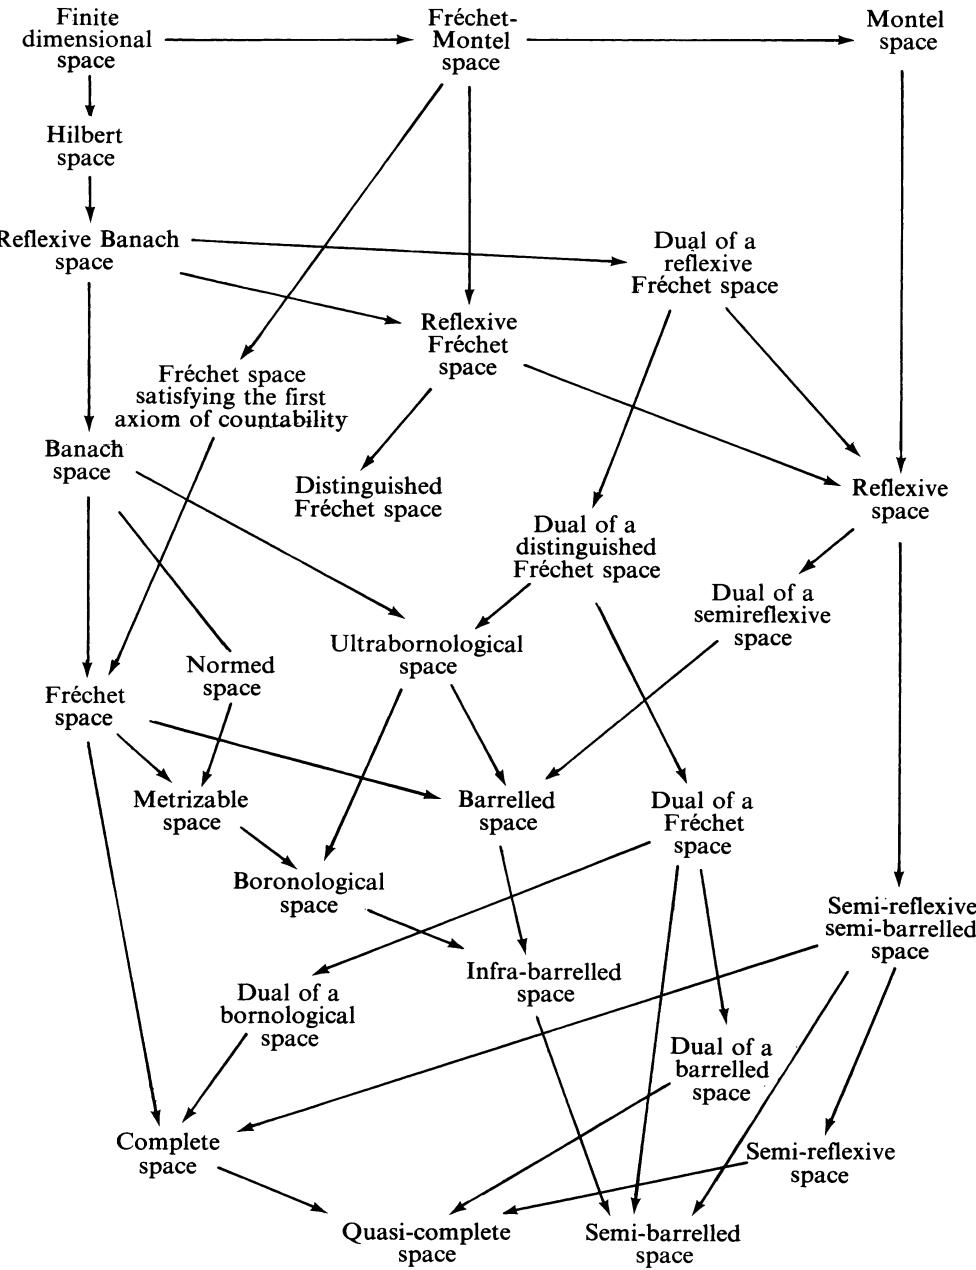
\includegraphics[keepaspectratio]{images/part002_27b26067.jpg}}

\bourbakitable{Principal bornologies on the dual of a locally convex space}{}
\pandocbounded{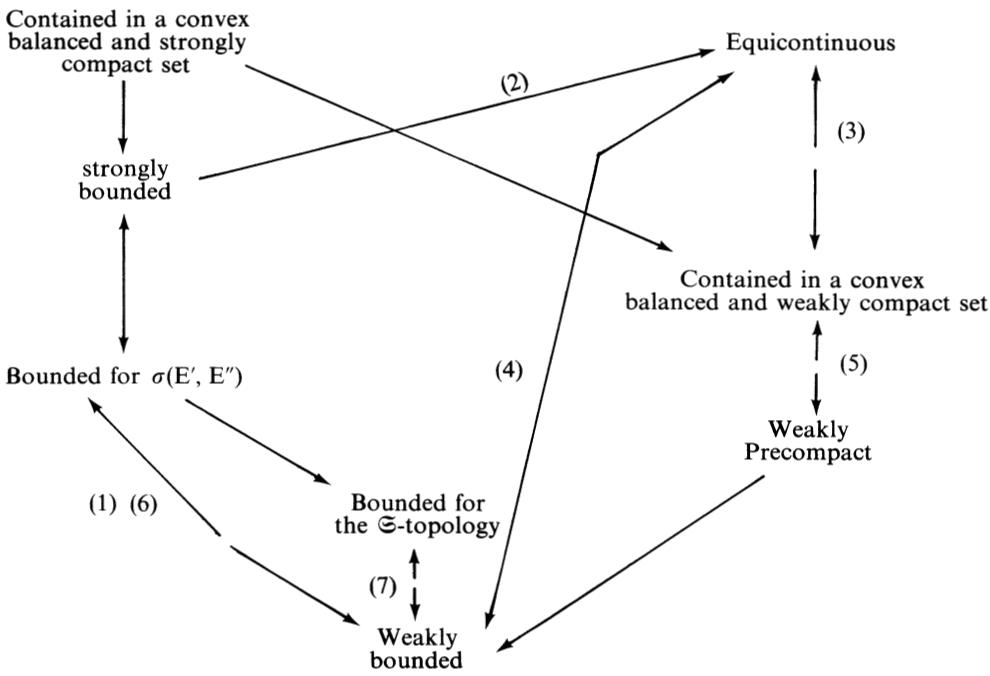
\includegraphics[keepaspectratio]{images/part002_d08e803b.jpg}}

N.B. --- We denote by S a family of bounded subsets of E such that every element is contained in a set belonging to S. A number on the side of an arrow indicates that the corresponding implication holds if the property with the same number is satisfied.

\paragraph{Properties}

\begin{enumerate}
\def\labelenumi{\arabic{enumi})}
\item
  Whenever E is semi-reflexive;
\item
  whenever E is bornological (III, p.~22, prop. 10);
\item
  if and only if E has the Mackey topology \(\tau(\mathrm{E},\mathrm{E}^{\prime})\) ;
\item
  if and only if E is barrelled;
\item
  if and only if \(\mathbf{E}'\) is quasi-complete for \(\sigma (\mathbf{E}',\mathbf{E})\)
\item
  whenever E is semi-complete (a fortiori, quasi-complete or complete) (III, p.~27, cor. 1);
\item
  whenever \(\mathfrak{S}\) consists of sets whose closed convex balanced envelope is semi-complete (III, p.~27, th. 2).
\end{enumerate}

When E is a Montel space, all the preceding bornologies are identical.

\chapter{\texorpdfstring{Hilbertian spaces \(^{1}\) (elementary theory)}{Hilbertian spaces \^{}\{1\} (elementary theory)}}

Throughout this chapter, K denotes the field R or the field C. For every complex number \(\xi = \alpha + i\beta (\alpha, \beta \text{ real}), \overline{\xi}\) denotes the conjugate \(\alpha - i\beta\) of \(\xi\) ; in particular, we have \(\overline{\xi} = \xi\) if and only if \(\xi\) is real.

\section{PREHILBERTIAN SPACES AND HILBERTIAN SPACES}

\subsection{Hermitian forms}

We recall the following definition given in Algebra (A, IX, § 3, No.~1):

DEFINITION 1. --- Let E be a vector space over the field K. A hermitian form (on the left) on E is a map f from E × E into K satisfying the following conditions (for \(x_{1}\) , \(x_{2}\) , x, \(y_{1}\) , \(y_{2}\) , y in E and \(\lambda\) , \(\mu\) in K):

\begin{enumerate}
\def\labelenumi{(\arabic{enumi})}
\tightlist
\item
\item
\end{enumerate}

\[
\begin{array}{c} \left\{ \begin{array}{l} f (x _ {1} + x _ {2}, y) = f (x _ {1}, y) + f (x _ {2}, y) \\ f (x, y _ {1} + y _ {2}) = f (x, y _ {1}) + f (x, y _ {2}) \end{array} \right. \\ \left\{ \begin{array}{l} f (\lambda x, y) = \overline {{\lambda}} f (x, y) \\ f (x, \mu y) = \mu f (x, y) \\ f (x, y) = \overline {{f (y , x)}}  . \end{array} \right. \end{array}\tag{3}
\]

When the field K is R, the notion of hermitian form on E reduces to that of symmetric bilinear form on \(E \times E\) (A, III, § 6, No.~3).

We note that the second condition (1) and the second condition (2) follow from the other three.

From (1) and (2) we deduce immediately that

\[
f \left(\sum_ {j} \lambda_ {j} x _ {j}, \sum_ {k} \mu_ {k} y _ {k}\right) = \sum_ {j, k} \bar {\lambda} _ {j} \mu_ {k} f \left(x _ {j}, y _ {k}\right).\tag{4}
\]

In particular, if \(\mathbf{E}\) is finite dimensional, and if \((e_j)_{1 \leqslant j \leqslant n}\) is a basis of \(\mathbf{E}\) , then for \(x = \sum_{j=1}^{n} \xi_j e_j\) and \(y = \sum_{j=1}^{n} \eta_j e_j\) , we have,

\[
f (x, y) = \sum_ {j, k} \alpha_ {j k} \overline {{{{\xi}}}} _ {j} \eta_ {k}
\]

with the notation \(\alpha_{jk} = f(e_j, e_k)\) ; moreover, relation (3) amounts to \(\alpha_{jk} = \overline{\alpha_{kj}}\) for every pair of indices \(j, k\) ; this implies in particular that the numbers \(\alpha_{jj}\) are real.

From (3), the number \(Q(x) = f(x, x)\) is real for all \(x \in E\) . Moreover, we immediately establish the following formulas, known as polarization formulas

\begin{enumerate}
\def\labelenumi{(\arabic{enumi})}
\setcounter{enumi}{4}
\tightlist
\item
\end{enumerate}

\[
4 f (x, y) = \sum_ {\varepsilon^ {2} = 1} \varepsilon \mathrm{Q} (x + \varepsilon y) \quad \text { if } \quad \mathbf {K} = \mathbf {R},\tag{6}
\]

\[
4 f (x, y) = \sum_ {\varepsilon^ {4} = 1, \varepsilon \in \mathbf {C}} \varepsilon \mathrm{Q} (x + \overline {{{\varepsilon}}} y) \quad \text { if } \quad \mathbf {K} = \mathbf {C}.
\]

Remark. --- We observe that formula (6) is valid for every sesquilinear form on \(E \times E\) (that is to say, for every function f satisfying (1) and (2), but not necessarily (3)). This remark shows that, when K = C, a sesquilinear form f such that \(f(x, x)\) is real for all \(x \in E\) is necessarily hermitian: relation (6) then gives \(\overline{f(y, x)} = f(x, y)\) since we have \(y + \varepsilon x = \varepsilon(x + \overline{\varepsilon}y)\) and \(\mathbf{Q}(\varepsilon z) = \mathbf{Q}(z)\) whenever \(\varepsilon^{4} = 1\) .

From the polarisation formulas, we have in particular,

PROPOSITION 1. --- If \(f\) is a hermitian form on \(\mathbf{E}\) , and \(\mathbf{M}\) a vector subspace of \(\mathbf{E}\) such that \(f(x, x) = 0\) for all \(x \in \mathbf{M}\) , then we also have \(f(x, y) = 0\) for every pair of points \(x, y\) in \(\mathbf{M}\) .

Let \(f\) be a hermitian form on \(\mathbf{E}\) ; the set \(\mathbf{N}\) of all \(x \in \mathbf{E}\) such that \(f(x, y) = 0\) for all \(y \in \mathbf{E}\) is a vector subspace of \(\mathbf{E}\) . It follows from (3) that, if \(x_1 \equiv x_2 \pmod{\mathbf{N}}\) and \(y_1 \equiv y_2 \pmod{\mathbf{N}}\) , we have \(f(x_1, y_1) = f(x_2, y_2)\) ; hence, on the quotient space \(\mathrm{E/N}\) we define a sesquilinear form \(f\) by putting \(\dot{f}(\dot{x}, \dot{y}) = f(x, y)\) for all \(x \in \dot{x}\) and all \(y \in \dot{y}\) ; it is clear that \(\dot{f}\) is hermitian and that the relation \(\langle \dot{f}(\dot{x}, \dot{y}) = 0 \text{ for all } \dot{y} \in \mathrm{E/N} \rangle\) implies \(\dot{x} = 0 \text{ in } \mathrm{E/N}\) , in other words (A, IX) \(\dot{f}\) is separating. We say that \(f\) is the separating hermitian form associated with \(f\) .

\subsection{Positive hermitian forms}

DEFINITION 2. --- Let E be a vector space over the field K. A hermitian form f on E is said to be positive if \(f(x, x) \geqslant 0\) for all \(x \in E\) .

It is clear that hermitian forms on a vector space E form a vector space over the field R (but not over the field C, when K is C): in this space the positive hermitian forms constitute a pointed convex proper cone (II, p.~10) as a result of def. 2 and prop. 1.

PROPOSITION 2. --- If \(f\) is a positive hermitian form, we have

\[
\left| f (x, y) \right| ^ {2} \leqslant f (x, x) f (y, y)\tag{7}
\]

for every x and y in E (Cauchy-Schwarz inequality).

First assume that we have \(f(y, y) \neq 0\) . For every \(\xi \in \mathbf{K}\) , we have

\[
f (y, y) f (x + \xi y, x + \xi y) \geqslant 0
\]

which can be written as

\[
f (x, x) f (y, y) - | f (x, y) | ^ {2} + (\xi f (y, y) + \overline {{f (x , y)}}) (\bar {\xi} f (y, y) + f (x, y)) \geqslant 0.
\]

Replacing \(\xi\) by \(-\overline{f(x,y)} / f(y,y)\) in this inequality, we get (7). If \(f(x,x)\neq 0\) , we argue similarly.

Finally, if \(f(x, x) = f(y, y) = 0\) , we have \(f(x + \xi y, x + \xi y) \geqslant 0\) for all \(\xi \in \mathbf{K}\) , which can be written as

\[
\xi f (x, y) + \overline {{{{\xi f (x , y)}}}} \geqslant 0.
\]

Replacing \(\xi\) by \(-\overline{f(x,y)}\) in this inequality, we get \(-2|f(x,y)|^2 \geqslant 0\) , and therefore \(f(x,y) = 0\) ; we again get (7) in this case.

COROLLARY 1. --- If \(f\) is a positive hermitian form, the set \(\mathbf{N}\) of all \(x \in \mathbf{E}\) such that \(f(x, x) = 0\) coincides with the vector subspace of all \(x \in \mathbf{E}\) such that \(f(x, y) = 0\) for all \(y \in \mathbf{E}\) .

COROLLARY 2. --- For a positive hermitian form to be separating, it is necessary and sufficient that the relation \(x \neq 0\) implies \(f(x, x) > 0\) .

This follows immediately from cor. 1.

For every positive hermitian form f on E, the separating hermitian form associated with \(f(\mathrm{V}, \mathrm{p.~2})\) is evidently a positive hermitian form on E/N.

PROPOSITION 3. --- Let f be a positive hermitian form on E. Put

\[
p (x) = f (x, x) ^ {1 / 2}
\]

for all \(x \in \mathbb{E}\) . Then \(p\) is a semi-norm on \(\mathbb{E}\) , and is a norm if and only if \(f\) is separating. It is enough to prove the inequality \(p(x + y) \leqslant p(x) + p(y)\) . But we have

\[
f (x + y, x + y) = f (x, x) + f (y, y) + f (x, y) + \overline {{f (x , y)}}
\]

and, by Cauchy-Schwarz inequality

\[
\begin{array}{c} f (x + y, x + y) \leqslant f (x, x) + f (y, y) + 2 (f (x, x) f (y, y)) ^ {1 / 2} \\ = \bigl (f (x, x) ^ {1 / 2} + f (y, y) ^ {1 / 2} \bigr) ^ {2}. \end{array}\tag{8}
\]

Remarks. --- 1) Suppose \(f\) is positive and separating, and let \(x, y\) be two vectors \(\neq 0\) . The proof of Cauchy-Schwarz inequality shows that, if the two members of (7) are equal, then there exists a scalar \(\xi\) such that \(f(x + \xi y, x + \xi y) = 0\) , hence \(x + \xi y = 0\) , in other words, x and y are linearly dependent; the converse is immediate. The proof of inequality (8) shows that the equality \(p(x + y) = p(x) + p(y)\) is possible only if x and y are linearly dependent; if \(y = \lambda x\) , the preceding equality can be written as \(|1 + \lambda| = 1 + |\lambda|\) , and implies that \(\lambda\) is real and positive.

\begin{enumerate}
\def\labelenumi{\arabic{enumi})}
\setcounter{enumi}{1}
\tightlist
\item
  Let \(f\) be a positive hermitian form on \(\mathbf{E}\) , and let \(\mathbf{E}\) be assigned the semi-norm \(x \mapsto f(x, x)^{1/2}\) ; if \(\dot{f}\) is the positive, separating hermitian form defined on \(\mathrm{E/N}\) associated with \(f\) , then the normed space obtained by assigning the norm \(x \mapsto \hat{f}(\dot{x}, \dot{x})^{1/2}\) to \(\mathrm{E/N}\) is the normed space associated with \(\mathbf{E}\) (II, p.~5).
\end{enumerate}

DEFINITION 3. --- Let E be a vector space over the field K. A semi-norm p on E is said to be prehilbertian if there exists a positive hermitian form f on E such that \(p(x) = f(x, x)^{1/2}\) for all \(x \in E\) .

Observe that for a semi-norm p on E, there exists at most one positive hermitian form f such that \(p(x) = f(x, x)^{1/2}\) for all \(x \in E\) ; this follows from the polarization formulas (V, p.~2).

\subsection{Prehilbertian spaces}

DEFINITION 4. --- A prehilbertian space is a set E with the structure of a vector space over K and with a positive hermitian form. We say that E is a real (resp. complex) prehilbertian space when K is R (resp. K is C).

Examples. --- 1) The form \((\lambda, \mu) \mapsto \overline{\lambda}\mu\) defines a prehilbertian structure on K, said to be canonical. When K is considered as a prehilbertian space, we shall always mean, unless otherwise mentioned that it has this structure.

\begin{enumerate}
\def\labelenumi{\arabic{enumi})}
\setcounter{enumi}{1}
\tightlist
\item
  Let I be an interval (bounded or not) in R, and let E be the set of regulated functions (FVR, II, p.~4) defined on I with values in C, having compact support. It is clear
\end{enumerate}

that \(\mathbf{E}\) is a vector space over \(\mathbf{C}\) ; let \(f\) be the sesquilinear form \((x, y) \mapsto \int_{1}^{\infty} \overline{x(t)} y(t) dt\) ;

it is immediate that \(f\) is a positive hermitian form on \(E\) , and hence defines a prehilbertian structure on this space.

\begin{enumerate}
\def\labelenumi{\arabic{enumi})}
\setcounter{enumi}{2}
\tightlist
\item
  Let \(n \geqslant 0\) be an integer. We define a prehilbertian space structure on the space \(\mathbf{K}^n\) , by means of the hermitian form
\end{enumerate}

\[
(x, y) \mapsto \sum_ {j = 1} ^ {n} \overline {{{{x}}}} _ {j} y _ {j}
\]

(for \(x = (x_{1}, \ldots, x_{n})\) and \(y = (y_{1}, \ldots, y_{n})\) ). When \(\mathbf{K}\) is \(\mathbf{R}\) , we see that this is just the scalar product of two vectors of \(\mathbf{R}^{n}\) (GT, VI, § 2, No.~2).

* 4) Let \(\ell^2\) (or \(\ell^2(\mathbf{N})\) ) be the set of sequences \(x = (x_n)_{n \in \mathbb{N}}\) of elements of \(\mathbf{K}\) such that \(\sum_{n=0}^{\infty} |x_n|^2\) is finite. One can show that \(\ell^2\) is a vector subspace of \(\mathbf{K}^{\mathbf{N}}\) and define a pre-

hilbertian space structure on \(\ell^2\) by means of the hermitian form \((x, y) \mapsto \sum_{n=0}^{\infty} \overline{x}_n y_n\) (cf.~V, p.~18).

\begin{enumerate}
\def\labelenumi{\arabic{enumi})}
\setcounter{enumi}{4}
\tightlist
\item
  Let \(\mathbf{E}\) be a real prehilbertian space, \(f\) the corresponding symmetric bilinear form on \(\mathbf{E}\) . Let \(\mathrm{E}_{(\mathbf{C})}\) be the vector space complexification of \(\mathbf{E}\) ; we identify \(\mathbf{E}\) with a subset of \(\mathrm{E}_{(\mathbf{C})}\) by the map \(x \mapsto 1 \otimes x\) , in such a way that every element of \(\mathrm{E}_{(\mathbf{C})}\) can be written uniquely as \(x_1 + ix_2\) with \(x_1, x_2\) in \(\mathbf{E}\) . The map \(f\) extends uniquely to a hermitian form \(f_{(\mathbf{C})}\) on \(\mathrm{E}_{(\mathbf{C})}\) ; we have,
\end{enumerate}

\[
f _ {(\mathbf {C})} \left(x _ {1} + i x _ {2}, y _ {1} + i y _ {2}\right) = f \left(x _ {1}, y _ {1}\right) + f \left(x _ {2}, y _ {2}\right) + i \left(f \left(x _ {1}, y _ {2}\right) - f \left(x _ {2}, y _ {1}\right)\right).
\]

In particular, we have

\[
f _ {(\mathbf {C})} (x _ {1} + i x _ {2}, x _ {1} + i x _ {2}) = f (x _ {1}, x _ {1}) + f (x _ {2}, x _ {2}) \geqslant 0,
\]

hence \(f_{(\mathbf{C})}\) is positive. We say that \(\mathrm{E}_{(\mathbf{C})}\) , with \(f_{(\mathbf{C})}\) is the prehilbertian space complexification of \(\mathbf{E}\) .

Whenever only one prehilbertian space structure on a vector space E is under consideration, the value, for a pair \((x, y)\) of points of E, of the hermitian form which defines the said structure is denoted by \(\langle x|y\rangle_{E}\) or simply \(\langle x|y\rangle\) , if no confusion is likely to arise. This number is called the scalar product \(^{1}\) of x and y (scalar square of x if y = x). Two vectors x, y are said to be orthogonal if \(\langle x|y\rangle = 0\) . The function \(x \mapsto \|x\| = \langle x|x\rangle^{1/2}\) is a semi-norm on the vector space E (V, p.~3); a prehilbertian space is always considered with this semi-norm assigned to it (and consequently also with the corresponding topology and uniform structure).

With these notations, in a prehilbertian space E, the Cauchy-Schwarz inequality can be written as

\[
\left| \langle x | y \rangle \right| \leqslant \| x \|\cdot \| y \|.\tag{9}
\]

Consequently, the scalar product is a continuous sesquilinear form on \(\mathbf{E} \times \mathbf{E}\) (II, p.~5, prop. 4).

In order that E be Hausdorff, it is necessary and sufficient that \(x \mapsto \|x\|\) is a norm on E; in other words, that the hermitian form \((x, y) \mapsto \langle x | y \rangle\) is positive and separating; this is equivalent to saying that 0 is the only vector of E, which is orthogonal to itself.

According to general definitions (S, IV, § 1, No.~5), an isomorphism from a prehilbertian space E onto a prehilbertian space F is a bijective linear mapping u from E onto F such that

\[
\langle u (x) | u (y) \rangle = \langle x | y \rangle\tag{10}
\]

for every x and y in E. We deduce from this that \(\|u(x)\| = \|x\|\) for all \(x \in E\) , and u is evidently an isomorphism for the topological vector space structures of E and of F; if E and F are Hausdorff, u is an isometry from E onto F. Conversely, if u is a bijective linear mapping from E onto F, such that \(\|u(x)\| = \|x\|\) for all \(x \in E\) , the polarization formulas (V, p.~2) show that u is a prehilbertian space isomorphism from E onto F.

Let \(E\) be a complex prehilbertian space, and \(\langle x|y\rangle\) the scalar product in \(E\) . On the set \(E\) , we can define a second vector space structure with respect to \(C\) , taking the same law of the additive group and for the law of external composition \((\lambda, x) \mapsto \overline{\lambda}x\) (A, II, § 1, No.~13) for this vector space structure, \((x, y) \mapsto \langle y|x\rangle\) is a positive hermitian

\(^{1}\) It may happen sometimes that we write \((x|y)\) for \(\langle y|x\rangle\) . Observe that the formula (4) of V, p.~2, takes the following equivalent forms:

(4')

\[
\langle \sum_ {i} \lambda_ {i} x _ {i} | \sum_ {j} \mu_ {j} y _ {j} \rangle = \sum_ {i, j} \overline {{{{\lambda}}}} _ {i} \mu_ {j} \langle x _ {i} | y _ {j} \rangle .\tag{4"}
\]

\[
(\sum_ {i} \lambda_ {i} x _ {i} | \sum_ {j} \mu_ {j} y _ {j}) = \sum_ {i, j} \lambda_ {i} \overline {{\mu}} _ {j} (x _ {i} | y _ {j}).
\]

form. The prehilbertian space \(\overline{E}\) obtained by assigning this new vector space structure and the new hermitian form to E, is said to be conjugate to E. An isomorphism u from E onto \(\overline{E}\) is a semi-linear mapping from E onto itself (with respect to the automorphism \(\xi \mapsto \overline{\xi}\) of C) such that \(\langle u(y)|u(x)\rangle = \langle x|y\rangle\) or \(\langle u(x)|u(y)\rangle = \overline{\langle x|y\rangle}\) (for x, y in E); such a mapping is said to be a semi-automorphism of the prehilbertian space E.

If E is a prehilbertian space, M a vector subspace of E, the restriction of the scalar product \(\langle x|y\rangle\) to \(M \times M\) is a positive hermitian form on M, which then defines a prehilbertian space structure on M; we say that this structure is induced by the structure of E, or that M is a prehilbertian subspace of E.

\subsection{Hilbertian spaces}

DEFINITION 5. --- A hilbertian space (or Hilbert space) is a prehilbertian space which is Hausdorff and complete. We say that a norm on a vector space E (over K) is hilbertian if it is prehilbertian, and if the normed space E is complete.

If E is a hilbertian space and M a closed vector subspace of E, the prehilbertian space structure induced on M is in fact a hilbertian space structure. In this case we say that M, with the induced structure is a hilbertian subspace of E.

Examples. --- 1) The prehilbertian spaces defined in examples 1, 3, 4 of V, p.~4, are hilbertian spaces. On the other hand, the prehilbertian space defined in example 2 is neither Hausdorff, nor complete. The complexification of a hilbertian space is a hilbertian space.

* 2) Let X be a Hausdorff topological space and let \(\mu\) be a positive measure on X. Let \(L^2(X, \mu)\) be the space consisting of equivalence classes, for \(\mu\) , of all square \(\mu\) -integrable functions on X with values in C. This is a complex hilbertian space, whose scalar product is given by

\[
\langle f | g \rangle = \int_ {\mathrm{X}} \overline {{{f (x)}}} g (x) d \mu (x). *
\]

* 3) Let \(n \geqslant 1\) be an integer and let \(U\) be an open set in \(\mathbf{R}^n\) . Let \(\mu\) be the measure on \(U\) induced by the Lebesgue measure on \(\mathbf{R}^n\) , and put \(\mathcal{H}^0 = L^2(U, \mu)\) . Let \(\mathcal{H}^1\) denote the space of all functions \(f \in \mathcal{H}^0\) with the following property; for \(1 \leqslant i \leqslant n\) , there exists a function \(g_i \in \mathcal{H}^0\) such that

\[
\int_ {\mathrm{U}} g _ {i} (x) h (x) d \mu (x) = - \int_ {\mathrm{U}} f (x) \mathrm{D} _ {i} h (x) d \mu (x)
\]

for every function \(h\) of class \(\mathbf{C}^1\) with compact support in \(\mathbf{U}\) . The function \(g_i\) is defined uniquely up to equivalence with respect to \(\mu\) , and is denoted by \(\mathbf{D}_i f\) or \(\partial f / \partial x_i\) (ith partial derivative). By induction on the integer \(s \geqslant 1\) , we define \(\mathcal{H}^s\) as the set of all functions \(f \in \mathcal{H}^1\) such that \(D_i f \in \mathcal{H}^{s-1}\) for \(1 \leqslant i \leqslant n\) . We define a scalar product on \(\mathcal{H}^s\) by the formula

\[
\langle f | g \rangle = \sum_ {k = 0} ^ {s} \sum_ {1 \leqslant i _ {1} \leqslant \dots \leqslant i _ {k} \leqslant n} \int \overline {{{{\mathrm{D} _ {i _ {1}} \dots \mathrm{D} _ {i _ {k}} f}}}}. \mathrm{D} _ {i _ {1}} \dots \mathrm{D} _ {i _ {k}} g d \mu .
\]

Then \(\mathcal{H}^s\) is a complex hilbertian space, called Sobolev space of index \(s\) .

* 4) Let X be a differential variety of class \(\mathbf{C}^r\) (with \(r \geqslant 1\) ) pure of finite dimension \(n\) .

In the vector fibre space \(\Lambda^{n}\mathrm{T}(\mathrm{X})\) , let L be the complement of the zero section. For every real number \(\lambda \neq 0\) , the mapping \(u \mapsto \lambda u\) from \(\Lambda^{n}\mathrm{T}(\mathrm{X})\) into itself leaves L stable.

Let \(\alpha\) be a complex number. A complex valued function \(\omega\) on \(\mathbf{L}\) such that \(\omega (\lambda u) = |\lambda |^{\alpha}\omega (u)\) for \(u\in \mathbf{L}\) and any non-zero real number \(\lambda\) is called a density of order \(\alpha\) on \(\mathbf{X}\) . We say that a density \(\omega\) of order 1 is locally integrable if there exists an open cover \((\mathrm{U}_i)_{i\in \mathbf{I}}\) of \(\mathbf{X}\) , and for every \(i\in \mathbf{I}\) a system of coordinates \(\xi_i = (\xi_i^1,\dots,\xi_i^n)\) on \(\mathrm{U}_i\) and a complex valued function \(f_{i}\) on \(\xi_i(\mathrm{U}_i)\) satisfying the following conditions: a) The function \(f_{i}\) is locally integrable on the open set \(\xi_i(\mathrm{U}_i)\) of \(\mathbf{R}^n\) with respect to the Lebesgue measure \(\mu\) ;

\begin{enumerate}
\def\labelenumi{\alph{enumi})}
\setcounter{enumi}{1}
\tightlist
\item
  Let \(x \in \mathbf{U}_i\) ; if \((\partial_{1,i,x}, \ldots, \partial_{n,i,x})\) is the basis of \(\mathrm{T}_x\mathrm{X}\) associated to the system of coordinates \((\xi_i^1, \ldots, \xi_i^n)\) in \(\mathbf{U}_i\) we have
\end{enumerate}

\[
\omega \left(\partial_ {1, i, x} \wedge \dots \wedge \partial_ {n, i, x}\right) = f _ {i} \left(\xi_ {i} ^ {1} (x), \dots , \xi_ {i} ^ {n} (x)\right).
\]

Then, there exists one and only one measure \(\tilde{\omega}\) on \(\mathbf{X}\) such that for every \(i\in \mathrm{I}\) , the image under \(\xi_{i}\) of the restriction of \(\tilde{\omega}\) to \(\mathrm{U}_i\) is equal to the measure \(f_{i}.\mu\) (cf.~VAR, R, 10.4.3).

Let \(\mathcal{V}\) (resp. \(\mathcal{N}\) ) be the vector space of measurable densities \(\omega\) of order \(1/2\) such that the measure associated with the density \(|\omega|^2\) of order 1 is bounded (resp. null). Let \(\omega_1\) and \(\omega_2\) be in \(\mathcal{V}\) ; then \(\omega = \overline{\omega}_1\omega_2\) is a density of order 1, and the measure \(\tilde{\omega}\) associated with \(\omega\) is bounded; the number \(\int_{\mathbf{X}}\tilde{\omega}\) depends only on the classes \(\dot{\omega}_1\) and \(\dot{\omega}_2\) of \(\omega_1\) and \(\omega_2\) modulo \(\mathcal{N}\) and is denoted by \(\langle\omega_1|\omega_2\rangle\) or \(\langle\dot{\omega}_1|\dot{\omega}_2\rangle\) . Then the mapping \((\dot{\omega}_1,\dot{\omega}_2)\mapsto\langle\dot{\omega}_1|\dot{\omega}_2\rangle\) assigns a complex hilbertian space structure to the vector space \(\Omega_{1/2}(\mathbf{X})=\mathcal{V}/\mathcal{N}_{*}\) .

*5) Let D be the open disc with centre 0 and radius 1 in C. The Hardy space \(\mathrm{H}^2 (\mathbf{D})\) consists of all holomorphic functions \(f\colon \mathbf{D}\to \mathbf{C}\) for which

\[
\sup _ {0 <   \mathbf {R} <   1} \int_ {0} ^ {1} | f (\mathbf {R}. \mathbf {e} (\theta)) | ^ {2} d \theta <   + \infty .
\]

If \(f_{1}\) and \(f_{2}\) belong to \(\mathrm{H}^2 (\mathbf{D})\) , the limit

\[
\langle f _ {1} | f _ {2} \rangle = \lim _ {\mathbf {R} \rightarrow 1} \int_ {0} ^ {1} \overline {{{f _ {1} (\mathbf {R} . \mathbf {e} (\theta))}}}. f _ {2} (\mathbf {R}. \mathbf {e} (\theta)) d \theta
\]

exists; the mapping \((f_1, f_2) \mapsto \langle f_1 | f_2 \rangle\) assigns a complex hilbertian space structure to the vector space \(\mathbf{H}^2(\mathbf{D})\) .

For a function \(f: \mathbf{D} \to \mathbf{C}\) to belong to \(\mathbf{H}^2(\mathbf{D})\) , it is necessary and sufficient that there exists a sequence \((a_n)_{n \in \mathbb{N}}\) of complex numbers such that \(\sum_{n=0}^{\infty} |a_n|^2 < +\infty\) and that

\[
f (z) = \sum_ {n = 0} ^ {\infty} a _ {n} z ^ {n}
\]

for all \(z \in \mathbf{D}\) . Then we have \(\| f\|^2 = \sum_{n=0}^{\infty} |a_n|^2\) which gives an isomorphism from \(\mathrm{H}^2(\mathrm{D})\) onto the hilbertian space \(\ell^2\) (V, p.~4). *

Every Hausdorff prehilbertian space is isomorphic to an everywhere dense subspace of a hilbertian space determined up to an isomorphism. Precisely :

PROPOSITION 4. --- Let E be a Hausdorff prehilbertian space, \(\hat{E}\) the normed space completion of E(GT, IX, § 3, No.~3). The scalar product \((x, y) \mapsto \langle x|y \rangle\) extends by continuity to a positive and separating hermitian form on \(\hat{\mathbf{E}}\) , and defines a hilbertian space structure on \(\hat{\mathbf{E}}\) .

The existence of the extension of \((x, y) \mapsto \langle x|y \rangle\) to \(\hat{E} \times \hat{E}\) follows from the continuity of this sesquilinear form on \(E \times E\) (GT, III, §6, No.~5, th. 1). Moreover, this extension, which will also be denoted by \((x, y) \mapsto \langle x|y \rangle\) is a hermitian form and satisfies the relation \(\langle x|x\rangle = \|x\|^2\) , by virtue of the principle of extension of identities ( \(\|x\|\) being the norm on \(\hat{E}\) obtained by extending the norm on E by continuity); this proves that the relation \(\langle x|x\rangle = 0\) implies x = 0 in \(\hat{E}\) , hence that the form \((x, y) \mapsto \langle x|y \rangle\) is positive and separating, and consequently defines a hilbertian space structure on \(\hat{E}\) .

Q.E.D.

This hilbertian space is said to be the completion of the Hausdorff prehilbertian space E.

* Example 6. --- Let U be an open subset of \(\mathbf{R}^n\) ( \(n \geqslant 1\) ). Let \(\mathcal{C}_0^1(\mathrm{U})\) be the vector space of all functions of class \(\mathbf{C}^1\) with compact support in U. We define a Hausdorff prehilbertian space structure on \(\mathcal{C}_0^1(\mathrm{U})\) whose scalar product is given by

\[
\langle f | g \rangle = \sum_ {i = 1} ^ {n} \int_ {\mathrm{U}} \overline {{{{\mathbf {D} _ {i} f (x)}}}}. \mathbf {D} _ {i} g (x) d x.
\]

This prehilbertian space is not complete. Its completion is called the Dirichlet space associated with U. *

COROLLARY. --- Let V be a vector space over K and f a positive hermitian form on V. a) There exists a Hilbert space E and a linear mapping \(u:V \rightarrow E\) such that \(f(x,y) = \langle u(x)|u(y) \rangle\) for x, y in V, and such that \(u(V)\) is dense in E.

\begin{enumerate}
\def\labelenumi{\alph{enumi})}
\setcounter{enumi}{1}
\tightlist
\item
  If two pairs \((\mathbf{E}_{i}, u_{i})\) satisfy the conditions analogous to a), then there exists a unique isomorphism \(\phi\) from the Hilbert space \(E_{1}\) onto the Hilbert space \(E_{2}\) such that \(u_{2} = \phi \circ u_{1}\) .
\end{enumerate}

Let N be the set of all \(x \in V\) such that \(f(x, x) = 0\) . We define a positive and separating hermitian form on the space V/N by \(\langle \dot{x} | \dot{y} \rangle = f(x, y)\) for \(x \in \dot{x}\) and \(y \in \dot{y}\) . Let E be the hilbertian space completion of V/N and u the mapping \(x \mapsto x + N\) from V into E. Then the conditions of a) are satisfied.

Under the hypotheses of b), N is equal to the kernel of \(u_{1}\) and to that of \(u_{2}\) . Hence there exists a bijective linear mapping \(\phi_{0}\) from \(u_{1}(V)\) onto \(u_{2}(V)\) such that \(u_{2}(x) = \phi_{0}(u_{1}(x))\) for all \(x \in V\) . We verify immediately that \(\phi_{0}\) is an isomorphism of prehilbertian spaces, hence an isometry. Since \(u_{i}(V)\) is dense in \(E_{i}\) for i = 1, 2, \(\phi_{0}\) extends uniquely to an isometry \(\phi\) from \(E_{1}\) onto \(E_{2}\) , and b) follows.

We say that the hilbertian space \(\mathbf{E}\) is the separated completion of \(\mathbf{V}\) (for the form \(f\) ).

Example 7. --- Let G be a group (with unit element 1) and \(\pi\) a homomorphism from G into the group of automorphisms of a complex hilbertian space E; we say that \(\pi\) is a unitary representation of G in E. Let \(a \in E\) ; we put

\[
\phi (x) = \langle a | \pi (x). a \rangle
\]

for all \(x \in \mathbf{G}\) . Then \(\phi : \mathbf{G} \to \mathbf{C}\) is positive definite, in other words satisfies the relation :

(PD) For every \(\lambda_{1},\ldots,\lambda_{n}\) in C and \(x_{1},\ldots,x_{n}\) in G, we have

\[
\sum_ {i, j = 1} ^ {n} \overline {{\lambda}} _ {i} \lambda_ {j} \phi (x _ {i} ^ {- 1} x _ {j}) \geqslant 0.\tag{11}
\]

In fact, the first member of (11) is precisely \(\| \sum_{i=1}^{n} \lambda_i \pi(x_i). a \|^2\) .

Conversely, let \(\phi\) be a positive definite function on \(G\) . Let \(\mathbf{C}^{(G)}\) be the vector space of all functions with finite support on \(G\) . We define a hermitian form \(\Phi\) on \(G\) by

\[
\Phi (u, v) = \sum_ {x, y \in G} \overline {{u (x)}} v (y) \phi (x ^ {- 1} y)\tag{12}
\]

and the relation (PD) expresses the fact that \(\Phi\) is positive. By the corollary of prop. 4, there exists a hilbertian space \(E\) and a linear mapping \(\rho : \mathbf{C}^{(G)} \to E\) , with a dense image, such that

\[
\Phi (u, v) = \langle \rho (u) | \rho (v) \rangle \quad \text { for } \quad u, v \quad \text { in } \quad \mathbf {C} ^ {(G)}.\tag{13}
\]

For every \(x \in \mathbf{G}\) , let \(\gamma_x\) be the left translation by \(x\) in \(\mathbf{C}^{(\mathrm{G})}\) defined by \(\gamma_x u(y) = u(x^{-1}y)\) for \(u \in \mathbf{C}^{(\mathrm{G})}\) and \(y \in \mathbf{G}\) . We have \(\Phi(\gamma_x u, \gamma_x v) = \Phi(u, v)\) . Now apply assertion \(b\) of the corollary of prop. 4 to \(\rho\) and \(\rho \circ \gamma_x\) : there exists a unique automorphism \(\pi(x)\) of the hilbertian space \(E\) such that \(\rho \circ \gamma_x = \pi(x) \circ \rho\) . We see immediately that \(\pi\) is a homomorphism from \(G\) into the group of automorphisms of \(E\) .

Let \(\delta\) be the element of \(\mathbf{C}^{(\mathrm{G})}\) defined by \(\delta(1) = 1\) , \(\delta(x) = 0\) for \(x \neq 1\) in \(\mathbf{G}\) . We have \(u = \sum_{x \in \mathbf{G}} u(x) \cdot \gamma_x \delta\) for all \(u \in \mathbf{C}^{(\mathrm{G})}\) , and so \(\rho(u) = \sum_{x \in \mathbf{G}} u(x) \pi(x) \cdot a\) by putting \(a = \rho(\delta)\) . Formulas (12) and (13) imply that \(\phi(x) = \langle a | \pi(x) \cdot a \rangle\) for all \(x \in \mathbf{G}\) . We remark that the set of vectors \(\pi(x) \cdot a\) for all \(x \in \mathbf{G}\) , is total in \(\mathbf{E}\) .

\subsection{Convex subsets of a prehilbertian space}

If we calculate \(\|x - y\|^{2} = \langle x - y|x - y \rangle\) and \(\|x + y\|^{2} = \langle x + y|x + y \rangle\) for any two points x, y of a prehilbertian space E, we immediately get the « identity of the median »

\[
\left\| \frac {1}{2} (x + y) \right\| ^ {2} + \left\| \frac {1}{2} (x - y) \right\| ^ {2} = \frac {1}{2} (\| x \| ^ {2} + \| y \| ^ {2}).\tag{14}
\]

From this identity we deduce the following proposition :

\pandocbounded{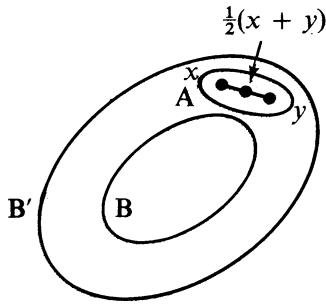
\includegraphics[keepaspectratio]{images/part002_56de9e6b.jpg}}\\
FIG. 1.

PROPOSITION 5. --- Let E be a prehilbertian space. Let d be a real number \textgreater0, δ a real number such that \(0 \leqslant \delta \leqslant d\) . Let B and B' be subsets of E defined by \(\|x\| < d\) , \(\| x\| \leqslant d + \delta\) respectively, and let A be a convex set contained in \(\mathbf{B}' - \mathbf{B}\) . Then for every pair of points \(x, y\) of A, we have \(\| x - y\| \leqslant \sqrt{12d\delta}\) (fig.~1).

In fact, we have \(\frac{1}{2} (x + y)\in \mathbf{A}\) , hence \(\| \frac{1}{2} (x + y)\| \geqslant d\) ; hence from (14) we get the inequality

\[
\left\| \frac {1}{2} (x - y) \right\| ^ {2} = \frac {1}{2} \left(\| x \| ^ {2} + \| y \| ^ {2}\right) - \left\| \frac {1}{2} (x + y) \right\| ^ {2} \leqslant (d + \delta) ^ {2} - d ^ {2} \leqslant 3 d \delta
\]

from which the proposition follows.

THEOREM 1. --- Let E be a prehilbertian space, and H a non-empty convex subset of E such that H is a Hausdorff and complete uniform subspace of E. For every \(x \in E\) , there exists a unique point \(p_{\mathrm{H}}(x)\) in H such that \(\|x - p_{\mathrm{H}}(x)\| = \inf_{y \in \mathrm{H}} \|x - y\|\) . The element \(p_{\mathrm{H}}(x)\) of H is also the unique element a of H satisfying the relation \(^{1}\)

\[
\mathcal {R} \langle x - a | y - a \rangle \leqslant 0\tag{15}
\]

for all \(y \in \mathbf{H}\) .

\pandocbounded{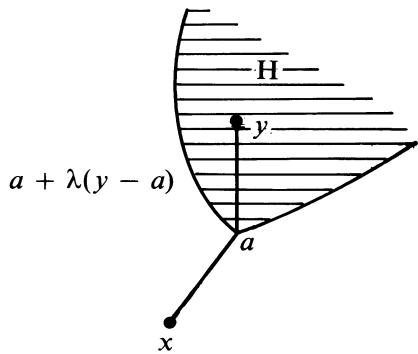
\includegraphics[keepaspectratio]{images/part002_6909685c.jpg}}\\
FIG. 2.

Put \(d = \inf_{y \in \mathbf{H}} \| x - y \|\) , and for every integer \(n > 0\) , let \(\mathrm{H}_n\) be the set of points \(y\) of \(\mathbf{H}\) such that \(\| x - y \| \leqslant d + n^{-1}\) . The set \(\mathrm{H}_n\) is closed in \(\mathbf{H}\) , is convex and non-empty, and its diameter is bounded by \(\sqrt{12d / n}\) for all large enough \(n\) , by prop. 5. The sequence \((\mathrm{H}_n)_{n \geqslant 1}\) being decreasing, and the set \(\mathbf{H}\) being Hausdorff and complete it follows that the base of the Cauchy filter \((\mathrm{H}_n)_{n \geqslant 1}\) converges to a point \(p_{\mathbf{H}}(x)\) of \(\mathbf{H}\) ; we have \(\{p_{\mathbf{H}}(x)\} = \bigcap_{n \geqslant 1} \mathrm{H}_n\) , hence \(p_{\mathbf{H}}(x)\) is the unique point \(a\) of \(\mathbf{H}\) such that \(\| x - a \| = d\) .

\(^{1}\) We recall (GT, VIII, § 1, No.~1) that \(\mathcal{R}(z)\) denotes the real part of the complex number z; we have \(\mathcal{R}(z)=z\) if z is real.

Let \(y \in H\) ; since \(H\) is convex, the point \(z(\lambda) = p_{\mathbf{H}}(x) + \lambda(y - p_{\mathbf{H}}(x))\) of \(E\) belongs to \(H\) for every real number \(\lambda\) such that \(0 < \lambda < 1\) . Hence we have

\[
\left\| x - z (\lambda) \right\| ^ {2} \geqslant \left\| x - p _ {\mathrm{H}} (x) \right\| ^ {2} \quad \text { for } \quad 0 <   \lambda <   1,
\]

which gives

\[
\mathcal {R} \left\langle x - p _ {\mathrm{H}} (x) \mid y - p _ {\mathrm{H}} (x) \right\rangle = \lim _ {\lambda \rightarrow 0} \frac {1}{2 \lambda} \left\{\| x - p _ {\mathrm{H}} (x) \| ^ {2} - \| x - z (\lambda) \| ^ {2} \right\} \leqslant 0.
\]

Conversely, let \(a\) be a point of \(\mathbf{H}\) such that \(\mathcal{R}\langle x - a|y - a\rangle \leqslant 0\) for all \(y\in \mathbf{H}\) . For every \(y\in \mathbf{H}\) , we have

\[
\left\| x - y \right\| ^ {2} = \left\| x - a \right\| ^ {2} + \left\| y - a \right\| ^ {2} - 2 \mathcal {R} \langle x - a | y - a \rangle \geqslant \left\| x - a \right\| ^ {2},
\]

and so \(\| x - a\| = d\) and finally that \(a = p_{\mathrm{H}}(x)\) follows from the first part of the proof. Q.E.D.

In what follows the mapping \(p_{H}\) of E in H will be called the projection from E onto H. We remark that \(p_{\mathrm{H}}(x)=x\) for all \(x\in H\) .

The first part of th. 1 is valid under more general hypotheses on the space E (V, p.~67, exerc. 31).

The proof of th. 1 establishes, among others, the following property :

COROLLARY 1. --- Let I be a set directed by a filter \(\mathfrak{F}\) and let \((y_i)_{i\in I}\) be a family of points of H. Let \(x\in E\) . Suppose that we have

\[
\lim _ {i, \mathfrak {F}} \| x - y _ {i} \| = \inf _ {z \in \mathrm{H}} \| x - z \|.
\]

Then \(y_{i}\) tends to \(p_{\mathrm{H}}(x)\) with respect to the filter \(\mathfrak{F}\) .

COROLLARY 2. --- For every x, y in E, we have

\[
\left\| p _ {\mathrm{H}} (x) - p _ {\mathrm{H}} (y) \right\| \leqslant \left\| x - y \right\|.
\]

In particular, the mapping \(p_{H}\) from E into H is continuous.

Let \(x, y\) be two points of \(E\) . Put \(a = p_{\mathrm{H}}(x) - x\) , \(b = p_{\mathrm{H}}(y) - p_{\mathrm{H}}(x)\) , \(c = y - p_{\mathrm{H}}(y)\) . By formula (15) (V, p.~10) we have \(\mathcal{R}\langle a|b\rangle \geqslant 0\) and \(\mathcal{R}\langle c|b\rangle \geqslant 0\) . We also have \(a + b + c = y - x\) , which gives,

\[
\| x - y \| ^ {2} = \| a + b + c \| ^ {2} = \| b \| ^ {2} + \| a + c \| ^ {2} + 2 \mathscr {R} \langle a | b \rangle + 2 \mathscr {R} \langle c | b \rangle
\]

\[
\geqslant \| b \| ^ {2} = \left\| p _ {\mathrm{H}} (x) - p _ {\mathrm{H}} (y) \right\| ^ {2}.
\]

This proves corollary 2.

PROPOSITION 6. --- Let E be a prehilbertian space and let \(\Phi\) be a non-empty, directed decreasing set of non-empty Hausdorff and complete convex subsets of E. For every \(x \in \mathrm{E}\) and every subset H of E, put \(d(x, \mathrm{H}) = \inf_{z \in \mathrm{H}} \| x - z \|\) . In order that the intersection M of the sets H belonging to \(\Phi\) be non-empty, it is necessary and sufficient that there exists \(x_0\) in E such that \(\sup_{\mathbf{H} \in \Phi} d(x_0, \mathbf{H})\) is finite. For every \(x \in \mathbf{E}\) we then have

\(p_{\mathbf{M}}(x) = \lim_{\mathrm{H}\in \Phi}p_{\mathrm{H}}(x)\) (limit with respect to the directed set \(\Phi\) ).

If \(\mathbf{M}\) is non-empty, \(d(x,\mathrm{H})\leqslant d(x,\mathbf{M})\) for all \(\mathbf{H}\in \Phi\) and all \(x\in \mathbb{E}\) .

Conversely, suppose that there exists a point \(x_0\) in \(\mathbf{E}\) and a real number \(\mathbf{C} \geqslant 0\) such that \(d(x_0, \mathbf{H}) \leqslant \mathbf{C}\) for all \(\mathbf{H} \in \Phi\) . Let \(x \in \mathbf{E}\) ; then

\[
d (x, \mathrm{H}) \leqslant \| x - x _ {0} \| + \mathrm{C} \quad \text { for   all } \quad \mathrm{H} \in \Phi ,
\]

hence the number \(d = \sup_{\mathbf{H} \in \Phi} d(x, \mathbf{H})\) is finite. Let \(\mathbf{B}\) be the set of all \(z \in E\) such that \(\| x - z\| \leqslant d\) . Since \(\mathbf{B}\) is convex and closed in \(\mathbf{E}\) , the sets \(\mathrm{H} \cap \mathrm{B}\) , for \(\mathrm{H}\) ranging over \(\Phi\) , are convex, Hausdorff and complete. Let \(\varepsilon > 0\) ; there exists a set \(\mathrm{H} \in \Phi\) such that \(d(x, \mathrm{H}) \geqslant \mathrm{d} - \varepsilon\) , and if \(\varepsilon < d/2\) , the diameter of \(\mathrm{H} \cap \mathrm{B}\) is bounded by \(\sqrt{12\varepsilon(d - \varepsilon)}\) by prop. 5 (V, p.~9). In other words, for all \(\mathrm{H}_0 \in \Phi\) , the closed sets \(\mathrm{H} \cap \mathrm{B}\) , for \(\mathrm{H} \in \Phi\) and \(\mathrm{H} \subset \mathrm{H}_0\) , form a base of the Cauchy filter on the Hausdorff and complete space \(\mathrm{H}_0\) . Hence the intersection of the sets \(\mathrm{H} \cap \mathrm{B}\) (for \(\mathrm{H} \in \Phi\) ) reduces to a point \(y\) . We get \(y \in \mathbf{M}\) and \(\| x - y \| = d = d(x, \mathbf{M})\) . Since \(\mathbf{M}\) is closed in \(\mathrm{H}_0\) , it is a Hausdorff, convex and complete set in \(\mathbf{E}\) , and so \(y = p_{\mathbf{M}}(x)\) . For every \(\mathrm{H} \in \Phi\) , we have \(p_{\mathrm{H}}(x) \in \mathrm{H} \cap \mathrm{B}\) , from which we get that \(p_{\mathbf{M}}(x) = \lim_{\mathrm{H} \in \Phi} p_{\mathrm{H}}(x)\) .

PROPOSITION 7. --- Let E be a Hausdorff prehilbertian space and let \(\Psi\) be a non-empty directed increasing set of non-empty, convex, complete subsets of E. Put \(A = \bigcup_{H \in \Psi} H\)

and suppose that the closure \(\mathbf{N}\) of \(\mathbf{A}\) is complete. Then \(\mathbf{N}\) is convex and we have \(p_{\mathrm{N}}(x) = \lim_{\mathrm{H}\in \Psi}p_{\mathrm{H}}(x)\) for all \(x\in \mathrm{E}\) .

It is clear that A is convex, hence its closure N is convex (II, p.~13). With the notations of prop. 6, \(d(x, \mathrm{N}) = \inf_{\mathrm{H} \in \Psi} d(x, \mathrm{H})\) , and consequently \(d(x, \mathrm{N})\) is the limit of \(d(x, \mathrm{H})\) with respect to the section filter of \(\Psi\) . Since \(p_{\mathrm{H}}(x) \in \mathrm{H}\) and

\[
\lim _ {\mathrm{H} \in \Psi} \| x - p _ {\mathrm{H}} (x) \| = \lim _ {\mathrm{H} \in \Psi} d (x, \mathrm{H}) = d (x, \mathrm{N}),
\]

it follows from cor. 1 of V, p.~11 that \(p_{\mathrm{H}}(x)\) tends to the projection \(p_{\mathrm{N}}(x)\) of \(x\) onto \(\mathbf{N}\) with respect to the section filter of \(\Psi\) .

\subsection{Vector subspaces and orthoprojectors}

Let \(\mathbf{E}\) be a prehilbertian space. Recall that two vectors \(x\) and \(y\) of \(\mathbf{E}\) are said to be orthogonal if \(\langle x|y\rangle = 0\) ; then

\[
\| x + y \| ^ {2} = \| x \| ^ {2} + \| y \| ^ {2}\tag{16}
\]

(« Pythagoras' theorem »).

Let A be a subset of E. We say that a vector x in E is orthogonal to A if it is orthogonal to every vector of A. The set of all vectors orthogonal to A is a closed vector subspace of A, denoted by \(A^{\circ}\) and called (by abuse of language) the orthogonal of A.

Let A and B be two subsets of E. We say that A and B are orthogonal if every vector of A is orthogonal to every vector of B. This is equivalent to saying that \(A \subset B^{\circ}\) , or that \(B \subset A^{\circ}\) . If E is Hausdorff and if A and B are orthogonal then \(A \cap B\) is empty or reduces to 0 since 0 is the only vector of E orthogonal to itself.

THEOREM 2. --- Let E be a prehilbertian space and M a vector subspace of E, which is Hausdorff and complete. Then E is the topological direct sum of M and of \(M^{\circ}\) the subspace orthogonal to M. The projector from E onto M associated with the decomposition \(E = M \oplus M^{\circ}\) is the projection \(p_{M}\) from E onto M defined in th. 1(V, p.~10).

We first show that \(x - p_{\mathbf{M}}(x)\) belongs to \(M^{\circ}\) for all \(x \in E\) . Let \(y \in M\) . For every scalar \(\lambda \in K\) , the vector \(p_{\mathbf{M}}(x) + \lambda y\) belongs to M; hence by formula 15 (V, p.~10) we have,

\[
\mathcal {R} \big (\lambda \langle x - p _ {\mathrm{M}} (x) | y \rangle \big) \leqslant 0
\]

for all \(\lambda \in \mathbf{K}\) . If, in particular we take \(\lambda = \overline{\langle x - p_{\mathbf{M}}(x)|y\rangle}\) we conclude that \(\langle x - p_{\mathbf{M}}(x)|y\rangle = 0\) , hence our assertion.

Since M is Hausdorff, 0 is the only vector of M, orthogonal to itself, hence \(M \cap M^{\circ} = \{0\}\) . For every \(x \in E\) , we have \(p_{\mathbf{M}}(x) \in \mathbf{M}\) and \(x - p_{\mathbf{M}}(x) \in \mathbf{M}^{\circ}\) . Consequently, E is the direct sum of M and \(M^{\circ}\) , and \(p_{M}\) is the projector from E onto M with kernel \(M^{\circ}\) . Since \(p_{M}\) is a continuous mapping from E into M (V, p.~11, cor. 2), it follows from GT, III, §6, No.~2 that E is the topological direct sum of M and \(M^{\circ}\) .

COROLLARY. --- Let E be a Hausdorff prehilbertian space and M a finite dimensional vector subspace of E. Then E is the direct sum of M and M°.

Since E is Hausdorff, so is M; since M is finite dimensional, it is complete (I, p.~13). It is therefore enough to apply th. 2.

With the notations of th. 2, we say that \(\mathbf{M}^{\circ}\) is the orthogonal complement of \(\mathbf{M}\) and that \(p_{\mathbf{M}}\) is the orthoprojector (or the orthogonal projector, or by abuse of language, the projector) from E onto \(\mathbf{M}\) ; if \(x\) is a vector of E, the vector \(p_{\mathbf{M}}(x)\) of \(\mathbf{M}\) is also called the orthogonal projection of \(x\) on \(\mathbf{M}\) . Note that \(p_{\mathbf{M}}\) is a continuous linear mapping from E onto \(\mathbf{M}\) and that we have \(\| p_{\mathbf{M}} \| = 1\) by cor. 2 of V, p.~11, except in the case when \(\mathbf{M} = \{0\}\) in which case \(p_{\mathbf{M}} = 0\) .

It follows immediately from Pythagoras theorem that the canonical mapping \(\psi\) from E/M onto \(M^{\circ}\) deduced from the direct sum decomposition \(E = M \oplus M^{\circ}\) is isometric if E/M is assigned the quotient semi-norm from that of E (II, p.~4). We shall always assign that prehilbertian structure to E/M for which \(\psi\) is an isomorphism of prehilbertian spaces; the quotient semi-norm on E/M is then deduced from this prehilbertian structure.

We shall often use the preceding results when E is a hilbertian space and M a closed vector subspace of E. In this case, \(M^{\circ}\) is a closed vector subspace of E, and \(p_{M^{\circ}} = 1 - p_{M}\) , and \((\mathbf{M}^{\circ})^{\circ} = \mathbf{M}\) .

PROPOSITION 8. --- Let E be a hilbertian space, M a closed vector subspace of E, I a non-empty ordered directed set and \((\mathbf{M}_{i})_{i\in I}\) a family of closed vector subspaces of E. We assume that either the mapping \(i\mapsto M_{i}\) is increasing and that M is the closure of \(\bigcup_{i\in I}M_{i}\) or that the mapping \(i\mapsto M_{i}\) is decreasing and that \(M=\bigcap_{i\in I}M_{i}\) . Then

\[
p _ {\mathbf {M}} (x) = \lim _ {i \in \mathbf {I}} p _ {\mathbf {M} _ {i}} (x)
\]

\[
x \in \mathrm{E}
\]

Prop. 8 follows immediately from props. 6 (V, p.~11) and 7 (V, p.~12).

PROPOSITION 9. --- Let E be a hilbertian space and M, N two closed vector subspaces of E.

\begin{enumerate}
\def\labelenumi{\alph{enumi})}
\tightlist
\item
  The following conditions are equivalent :
\end{enumerate}

\begin{enumerate}
\def\labelenumi{(\roman{enumi})}
\item
  \(p_{\mathbf{M}}p_{\mathbf{N}} = p_{\mathbf{N}}p_{\mathbf{M}}\)
\item
  if \(x \in \mathbf{M}\) is orthogonal to \(\mathbf{M} \cap \mathbf{N}\) and if \(y \in \mathbf{N}\) is orthogonal to \(\mathbf{M} \cap \mathbf{N}\) , then \(x\) and \(y\) are orthogonal;
\item
  every vector of M orthogonal to \(\mathbf{M} \cap \mathbf{N}\) is orthogonal to \(\mathbf{N}\) ;
\item
  \(\mathbf{M} = (\mathbf{M}\cap \mathbf{N}) + (\mathbf{M}\cap \mathbf{N}^{\circ}).\)
\end{enumerate}

\begin{enumerate}
\def\labelenumi{\alph{enumi})}
\setcounter{enumi}{1}
\item
  If the equivalent conditions of a) are satisfied, we have \(p_{M \cap N} = p_{M} p_{N}\) , the vector subspace M + N of E is closed and we have \(p_{M + N} = p_{M} + p_{N} - p_{M} p_{N}\) .
\item
  We have \(p_{\mathbf{M}}p_{\mathbf{N}} = 0\) if and only if \(\mathbf{M}\) is orthogonal to \(\mathbf{N}\) . If this is so, then the vector subspace \(\mathbf{M} + \mathbf{N}\) of \(\mathbf{E}\) is closed, and \(p_{\mathbf{M} + \mathbf{N}} = p_{\mathbf{M}} + p_{\mathbf{N}}\) .
\end{enumerate}

Put \(L = M \cap N\) , \(M_{1} = M \cap L^{\circ}\) and \(N_{1} = N \cap L^{\circ}\) . Condition (ii) implies that \(M_{1}\) and \(N_{1}\) are orthogonal, and (iii) implies that \(M_{1}\) and N are orthogonal. Since we have \(N = N_{1} + L\) and \(M_{1}\) is orthogonal to L, we have proved the equivalence of (ii) and (iii). If condition (iii) is satisfied, we have \(M_{1} = M \cap N^{\circ}\) and since \(M = L + M_{1}\) , condition (iv) is satisfied. Conversely, from (iv) we conclude that \(M_{1} = M \cap N^{\circ}\) since the subspaces \(M \cap N\) and \(M \cap N^{\circ}\) of M are orthogonal, and so \(M_{1} \subset N^{\circ}\) , that is, the relation (iii).

Assume that condition (iv) is satisfied. It is immediate that \(p_{\mathbf{N}}(y) = p_{\mathbf{L}}(y)\) for all \(y \in M\) and hence \(p_{\mathbf{N}}p_{\mathbf{M}}(x) = p_{\mathbf{L}}p_{\mathbf{M}}(x)\) for all \(x \in E\) . But, for every \(x \in E\) , the vector \(p_{\mathbf{L}}p_{\mathbf{M}}(x)\) belongs to L, and the vector

\[
x - p _ {\mathrm{L}} p _ {\mathrm{M}} (x) = \left(x - p _ {\mathrm{M}} (x)\right) + \left(p _ {\mathrm{M}} (x) - p _ {\mathrm{L}} \left(p _ {\mathrm{M}} (x)\right)\right)
\]

belongs to \(\mathbf{M}^{\circ} + \mathbf{L}^{\circ} = \mathbf{L}^{\circ}\) ; hence we have \(p_{\mathrm{L}}p_{\mathrm{M}}(x) = p_{\mathrm{L}}(x)\) . Finally, \(p_{\mathrm{N}}p_{\mathrm{M}} = p_{\mathrm{L}}p_{\mathrm{M}} = p_{\mathrm{L}}\) . Since condition (ii) is equivalent to (iv) and is symmetric in \(\mathbf{M}\) and \(\mathbf{N}\) , we also have \(p_{\mathrm{M}}p_{\mathrm{N}} = p_{\mathrm{L}}\) . Finally we get \(p_{\mathrm{M}}p_{\mathrm{N}} = p_{\mathrm{N}}p_{\mathrm{M}} = p_{\mathrm{M}\cap \mathrm{N}}\) which gives (i).

Conversely, suppose condition (i) is satisfied. Let \(x \in M\) ; we have

\[
p _ {\mathbf {M}} (p _ {\mathbf {N}} (x)) = p _ {\mathbf {N}} (p _ {\mathbf {M}} (x)) = p _ {\mathbf {N}} (x)
\]

and so \(p_{\mathbf{N}}(x) \in \mathbf{M}\) . We conclude that \(x - p_{\mathbf{N}}(x) \in \mathbf{M}\) , hence \(x\) is the sum of an element \(p_{\mathbf{N}}(x)\) of \(\mathbf{M} \cap \mathbf{N}\) and an element \(x - p_{\mathbf{N}}(x)\) of \(\mathbf{M} \cap \mathbf{N}^{\circ}\) , which gives (iv).

We have proved \(a)\) and the first part of \(b)\) . Assume now that \(p_{\mathbf{M}}\) and \(p_{\mathbf{N}}\) commute and put \(q = p_{\mathbf{M}} + p_{\mathbf{N}} - p_{\mathbf{M}}p_{\mathbf{N}}\) ; since \(p_{\mathbf{M}}\) and \(p_{\mathbf{N}}\) are idempotents in the algebra \(\mathcal{L}(\mathbf{E})\) , so is \(q\) ; hence (GT, III, § 6, No.~2) the image of \(q\) is a closed vector subspace of \(\mathbf{E}\) .

It is clear that the image of \(q\) is contained in \(\mathbf{M} + \mathbf{N}\) ; however, we have \(p_{\mathbf{N}}(x) = x\) , hence \(q(x) = x\) for all \(x \in \mathbf{N}\) ; since we also have \(q = p_{\mathbf{M}} + p_{\mathbf{N}} - p_{\mathbf{N}}p_{\mathbf{M}}\) , we get \(q(x) = x\) for all \(x \in \mathbf{M}\) . We conclude that the image of \(q\) is equal to \(\mathbf{M} + \mathbf{N}\) . The orthogonal of \(\mathbf{M} + \mathbf{N}\) is equal to \(\mathbf{M}^{\circ} \cap \mathbf{N}^{\circ}\) , and the kernel of \(q\) obviously contains \(\mathbf{M}^{\circ} \cap \mathbf{N}^{\circ}\) , hence \(q = p_{\mathbf{M} + \mathbf{N}}\) . This proves \(b\) .

We have \(p_{\mathbf{M}}p_{\mathbf{N}} = 0\) if and only if the image \(\mathbf{N}\) of \(p_{\mathbf{N}}\) is contained in the kernel \(\mathbf{M}^{\circ}\) of \(p_{\mathbf{M}}\) , that is, if and only if \(\mathbf{M}\) is orthogonal to \(\mathbf{N}\) . The rest of the assertion \(c)\) is then a particular case of \(b)\) .

Remark. --- Let E be a hilbertian space and M, N two closed vector subspaces of E. The relation \(M \subset N\) is equivalent to the orthogonality of M and \(N^{\circ}\) , that is to say, to the relation \(p_{M}p_{N^{\circ}} = 0\) by prop. 9, c). Since we have \(p_{N^{\circ}} = 1 - p_{N}\) , we conclude that the relations \(M \subset N\) and \(p_{M} = p_{M}p_{N}\) are equivalent (« the three perpendicular theorem », cf.~fig.~3).

\pandocbounded{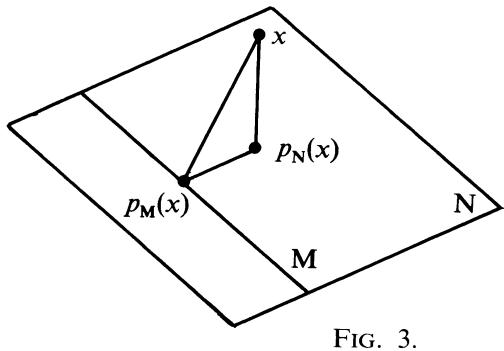
\includegraphics[keepaspectratio]{images/part002_dc4b20c6.jpg}}

\subsection{Dual of a hilbertian space}

THEOREM 3. --- Let E be a hilbertian space. For every \(x \in E\) , let \(x^{*}\) be the continuous linear form \(y \mapsto \langle x | y \rangle\) on E; the mapping \(x \mapsto x^{*}\) is a bijective, semi-linear (for the automorphism \(\xi \mapsto \overline{\xi}\) ) mapping from E onto its dual \(E'\) , and an isometry from the normed space E onto the normed space \(E'\) .

The mapping \(x \mapsto x^*\) is semi-linear by (2) (V, p.~1) and by virtue of the Cauchy-Schwarz inequality, we have \(\| x^* \| = \sup_{\| y \| \leqslant 1} |\langle x | y \rangle| = \| x \|\) , hence \(x \mapsto x^*\) is an isometry from E into E', and in particular, is injective. To complete the proof, we need to prove that for all \(x' \neq 0\) in E', there exists \(x \in E\) such that \(x' = x^*\) . But the hyperplane \(H = Ker x'\) is closed in E; its orthogonal is a line D. Let \(b\) be a non-zero element of D; the kernel of the linear form \(b^*\) is equal to H and hence there exists a scalar \(\lambda \neq 0\) such that \(x' = \lambda . b^* = (\overline{\lambda}. b)^*\) . Q.E.D.

The mapping \(x \mapsto x^{*}\) from E onto its dual \(E'\) is said to be canonical. The inverse mapping from \(E'\) onto E is also called canonical and is denoted by \(x' \mapsto x'^{*}\) . We have

\[
\langle x | y \rangle = \langle y, x ^ {*} \rangle , \quad \langle x, x ^ {\prime} \rangle = \langle x ^ {\prime *} | x \rangle\tag{17}
\]

for \(x, y\) in E and \(x'\) in E'. Also \((x^{*})^{*} = x\) for \(x \in \mathbf{E}\) .

When K is R, the mapping \(x \mapsto x^{*}\) is linear. We shall transfer the scalar product of E to \(E'\) by this mapping. When \(K = C\) , we can consider the mapping \(x \mapsto x^{*}\) as an isomorphism from the vector space \(\overline{E}\) , the conjugate of E onto \(E'\) (V, p.~6). We shall transfer the scalar product of \(\overline{E}\) to \(E'\) by this mapping.

In the two cases considered, \(E'\) is a hilbertian space and we have the formulae

\[
\langle x ^ {*} | y ^ {*} \rangle = \overline {{\langle x | y \rangle}}, \quad \langle x ^ {\prime} | x ^ {\prime} \rangle = \| x ^ {\prime} \| ^ {2}
\]

for \(x, y\) in \(\mathbf{E}\) and \(x'\) in \(\mathbf{E}'\) .

To say that the vector \(x \in E\) is orthogonal to a vector \(y \in E\) is equivalent to saying that the linear form \(x^{*} \in E'\) is orthogonal to y in the sense defined in II, p.~41 (this justifies the use of the word « orthogonal » in the two cases). If M is a closed vector subspace of E, the subspace \(M^{\circ}\) orthogonal to M in \(E'\) (II, p.~44) is the image under \(x \mapsto x^{*}\) of the orthogonal of M in E, defined in V, p.~13 (this justifies the use of the notation \(M^{\circ}\) in the two cases).

COROLLARY 1.--- In order that the family \((x_{i})_{i\in I}\) of points of a hilbertian space E be total, it is necessary and sufficient that the relations \(\langle x_{i}|y\rangle = 0\) for \(y \in E\) and for all indices \(i \in I\) imply that y = 0.

In fact, this says that 0 is the only vector of \(\mathbf{E}'\) which is orthogonal to all the \(x_{i}\) (II, p.~43 and IV, p.~1).

COROLLARY 2. --- Let E and F be two hilbertian spaces. For \(u \in \mathcal{L}(\mathrm{E};\mathrm{F})\) , \(x \in \mathrm{E}\) and \(y \in \mathrm{F}\) , put

\[
\Phi_ {u} (y, x) = \langle y | u (x) \rangle .\tag{18}
\]

The mapping \(u \mapsto \Phi_u\) is an isomorphism from the Banach space \(\mathcal{L}(\mathrm{E};\mathrm{F})\) onto the space of all continuous sesquilinear \(^1\) forms on \(\mathrm{F} \times \mathrm{E}\) , endowed with the norm

\[
\| f\| = \sup_{\substack{x\in \mathbf{E},  y\in \mathbf{F}\\ \| x\| \leqslant 1, \| y\| \leqslant 1}}\left|f(y,x)\right|.\tag{19}
\]

It is clear that \(\Phi_u\) is sesquilinear and continuous for all \(u \in \mathcal{L}(\mathrm{E};\mathrm{F})\) . Conversely, let \(f\) be a continuous sesquilinear form on \(\mathrm{F} \times \mathrm{E}\) . For every \(x \in \mathrm{E}\) , the mapping \(y \mapsto \overline{f(y,x)}\) is a continuous linear form on the hilbertian space \(\mathrm{F}\) . By th. 3, for every \(x \in \mathrm{E}\) , there exists a unique element \(u(x)\) in \(\mathrm{F}\) such that \(\overline{f(y,x)} = \langle u(x)|y\rangle\) for all \(y \in \mathrm{F}\) . The mapping \(u: x \mapsto u(x)\) from \(\mathrm{E}\) into \(\mathrm{F}\) is linear and we have

\[
\begin{array}{l} \| f \| = \sup _ {\| x \| \leqslant 1} \sup _ {\| y \| \leqslant 1} | f (y, x) | = \sup _ {\| x \| \leqslant 1} \sup _ {\| y \| \leqslant 1} | \langle y | u (x) \rangle | \\ = \sup _ {\| x \| \leqslant 1} \| u (x) \|; \end{array}
\]

hence \(u\) belongs to \(\mathcal{L}(\mathrm{E};\mathrm{F})\) , \(f = \Phi_u\) and \(\| u\| = \| f\|\) . This proves cor. 2.

\(^{1}\) Recall (A, IX, § 1, No.~5) that a sesquilinear form (on the left) f on F × E is a mapping from F × E into K which satisfies relations (1) and (2) of V, p.~1.

The canonical mapping from E into its bidual \(E''\) (IV, p.~14) maps E onto \(E''\) , in other words (IV, p.~16), E is a reflexive Banach space. In fact, if E is a real (resp. complex) hilbertian space, the canonical mapping \(\phi\) from \(E'\) onto E is an isomorphism from the normed space \(E'\) onto E (resp. onto the conjugate space \(\overline{E}\) of E); applying th. 3 to E (resp. \(\overline{E}\) ), we see that every continuous linear form on the normed space \(E'\) is of the form \(x' \mapsto \langle \phi(x') | x \rangle = \langle x, x' \rangle\) with \(x \in E\) , hence our assertion follows.

As a consequence (IV, p.~17, prop. 6):

THEOREM 4. --- In a hilbertian space E, the unit ball is weakly compact.

PROPOSITION 10. --- If, in a hilbertian space E, a filter F converges weakly to \(x_{0}\) , and if moreover \(\lim_{\mathfrak{F}} \|x\| = \|x_{0}\|\) , then F converges to \(x_{0}\) for the initial topology of E. In fact, \(\|x - x_{0}\|^{2} = \|x\|^{2} - 2R \langle x|x_{0} \rangle + \|x_{0}\|^{2}\) . Since \(\langle x|x_{0}\rangle\) tends to \(\|x_{0}\|^{2}\) with respect to F by hypothesis, and \(\|x\|\) tends to \(\|x_{0}\|\) with respect to F, \(\|x - x_{0}\|\) tends to 0 with respect to F, hence the proposition.

Remark. --- If E is a Hausdorff prehilbertian space and \(\hat{E}\) the hilbertian space completion of E, we know (III, p.~16) that the dual \(E'\) of E can be identified with the dual of \(\hat{E}\) ; it then follows from th. 3 (V, p.~15) that every continuous linear form on E can be written in a unique way as \(x \mapsto \langle a|x\rangle\) , where \(a \in \hat{E}\) .

\section{ORTHOGONAL FAMILIES IN A HILBERTIAN SPACE}
